% A LaTeX template for ARTICLE version of the MSc Thesis submissions to 
% Politecnico di Milano (PoliMi) - School of Industrial and Information Engineering
%
% S. Bonetti, A. Gruttadauria, G. Mescolini, A. Zingaro
% e-mail: template-tesi-ingind@polimi.it
%
% Last Revision: October 2021
%
% Copyright 2021 Politecnico di Milano, Italy. Inc. NC-BY

\documentclass[11pt,a4paper]{article} 

%------------------------------------------------------------------------------
%	REQUIRED PACKAGES AND  CONFIGURATIONS
%------------------------------------------------------------------------------
% PACKAGES FOR TITLES
\usepackage{titlesec}
\usepackage{color}

% PACKAGES FOR LANGUAGE AND FONT
\usepackage[utf8]{inputenc}
\usepackage[english]{babel}
\usepackage[T1]{fontenc} % Font encoding
\usepackage{newunicodechar}
\newunicodechar{≈}{\approx}

% PACKAGES FOR IMAGES
\usepackage{graphicx}
\usepackage{float}
\graphicspath{{Images/}}
\usepackage{eso-pic} % For the background picture on the title page
\usepackage{subfig} % Numbered and caption subfigures using \subfloat
\usepackage{caption} % Coloured captions
\usepackage{transparent}

% STANDARD MATH PACKAGES
\usepackage{amsmath}
\usepackage{amsthm}
\usepackage{bm}
\usepackage[overload]{empheq}  % For braced-style systems of equations

% PACKAGES FOR TABLES
\usepackage[utf8]{inputenc}
\usepackage{booktabs} % Per tabelle professionali
\usepackage{siunitx}  % Per unità di misura e simboli
\usepackage{tabularx}
\usepackage{longtable} % tables that can span several pages
\usepackage{colortbl}

% PACKAGES FOR ALGORITHMS (PSEUDO-CODE)
\usepackage{algorithm}
\usepackage{algorithmic}

% PACKAGES FOR REFERENCES & BIBLIOGRAPHY
\usepackage[colorlinks=true,linkcolor=black,anchorcolor=black,citecolor=black,filecolor=black,menucolor=black,runcolor=black,urlcolor=black]{hyperref} % Adds clickable links at references
\usepackage{cleveref}
\usepackage[square, numbers, sort&compress]{natbib} % Square brackets, citing references with numbers, citations sorted by appearance in the text and compressed
\bibliographystyle{plain} % You may use a different style adapted to your field

% PACKAGES FOR THE APPENDIX
\usepackage{appendix}

% PACKAGES FOR ITEMIZE & ENUMERATES 
\usepackage{enumitem}

% OTHER PACKAGES
\usepackage{amsthm,thmtools,xcolor} % Coloured "Theorem"
\usepackage{comment} % Comment part of code
\usepackage{fancyhdr} % Fancy headers and footers
\usepackage{lipsum} % Insert dummy text
\usepackage{tcolorbox} % Create coloured boxes (e.g. the one for the key-words)

%-------------------------------------------------------------------------
%	NEW COMMANDS DEFINED
%-------------------------------------------------------------------------
% EXAMPLES OF NEW COMMANDS -> here you see how to define new commands
\newcommand{\bea}{\begin{eqnarray}} % Shortcut for equation arrays
\newcommand{\eea}{\end{eqnarray}}
\newcommand{\e}[1]{\times 10^{#1}}  % Powers of 10 notation
\newcommand{\mathbbm}[1]{\text{\usefont{U}{bbm}{m}{n}#1}} % From mathbbm.sty
\newcommand{\pdev}[2]{\frac{\partial#1}{\partial#2}}
% NB: you can also override some existing commands with the keyword \renewcommand

%----------------------------------------------------------------------------
%	ADD YOUR PACKAGES (be careful of package interaction)
%----------------------------------------------------------------------------


%----------------------------------------------------------------------------
%	ADD YOUR DEFINITIONS AND COMMANDS (be careful of existing commands)
%----------------------------------------------------------------------------


% Do not change Configuration_files/config.tex file unless you really know what you are doing. 
% This file ends the configuration procedures (e.g. customizing commands, definition of new commands)
\input{Configuration_files/config}

% Insert here the info that will be displayed into your Title page 
% -> title of your work
\renewcommand{\title}{Pulse Arrival Time (PAT) per stima della pressione arteriosa}
% -> author name and surname
\renewcommand{\author}{Anna Carazza - 11094888, Andrea Guidi - 10798686, Matteo Gandini - 10751617, Giorgia Moroni - 10768555, Fabiola Maria Ribolsi - 10809720}
% -> MSc course
\newcommand{\course}{Laboratorio di Tecnologie Elettroniche e Biosensori}
% -> advisor name and surname
\newcommand{\advisor}{Prof. Alessandra Angelucci}
% IF AND ONLY IF you need to modify the co-supervisors you also have to modify the file Configuration_files/title_page.tex (ONLY where it is marked)
\newcommand{\firstcoadvisor}{Name Surname} % insert if any otherwise comment
\newcommand{\secondcoadvisor}{Name Surname} % insert if any otherwise comment
% -> author ID
% -> academic year
\newcommand{\YEAR}{2025-2026}
% -> abstract (only in English)
\renewcommand{\abstract}{Questo report presenta lo sviluppo di un progetto del corso di Laboratorio di Tecnologie Elettroniche e Biosensori tenuto nell'A.A. 2025-2026 presso il Politecnico di Milano. Si tratta della realizzazione di un sistema \textit{wearable} per la stima non invasiva della pressione arteriosa basato sul \textit{Pulse Arrival Time} (PAT), ottenuto dalla misura sincronizzata dei segnali ECG e PPG. L’architettura impiega due unità di acquisizione indipendenti, ciascuna basata su microcontrollore nRF52840 e dotata di \textit{Real Time Clock} dedicato, al fine di garantire un’elevata accuratezza temporale. I segnali acquisiti vengono trasmessi tramite Bluetooth Low Energy a un elaboratore esterno, che li analizza per individuare i punti fiduciali e calcolare il PAT. La stima della pressione arteriosa è ottenuta mediante modelli di regressione calibrati sul singolo utente, includendo anche la frequenza cardiaca per migliorare l’accuratezza.  
L’iter di sviluppo del sistema, dettagliato nei paragrafi successivi, comprende la progettazione dell'hardware e del firmware, il software di elaborazione dati, il design dei case, lo sviluppo di una \textit{Graphic User Interface} (GUI) dedicata e la proposta di un protocollo di validazione.
I risultati mostrano il potenziale del sistema per applicazioni di monitoraggio continuo \textit{Beat-to-Beat}, evidenziando al contempo i principali limiti legati alla sincronizzazione e alla deriva temporale.}

% -> key-words (only in English)
\newcommand{\keywords}{Pressione Arteriosa, BP, PAT, PTT, ECG, PPG, BPM}

%-------------------------------------------------------------------------
%	BEGIN OF YOUR DOCUMENT
%-------------------------------------------------------------------------
\begin{document}

%-----------------------------------------------------------------------------
% TITLE PAGE
%-----------------------------------------------------------------------------
% Do not change Configuration_files/TitlePage.tex (Modify it IF AND ONLY IF you need to add or delete the Co-advisors)
% This file creates the Title Page of the document
\input{Configuration_files/title_page}

%%%%%%%%%%%%%%%%%%%%%%%%%%%%%%
%%     THESIS MAIN TEXT     %%
%%%%%%%%%%%%%%%%%%%%%%%%%%%%%%

%-----------------------------------------------------------------------------
% INTRODUCTION
%-----------------------------------------------------------------------------
\section{Introduzione}
\label{sec:introduction}
\subsection{Contesto e Necessità}
L’incidenza sempre crescente delle malattie cardiovascolari (CVD) e la loro stretta correlazione con la pressione sanguigna (BP), unitamente alle limitazioni degli attuali metodi di misurazione, hanno reso necessario lo sviluppo e l’adozione di tecniche di misura non invasive \cite{Zhou2023}.
L'ipertensione, che rappresenta il fattore di rischio più comune per queste patologie, è spesso asintomatica, rendendo necessari strumenti che permettano un monitoraggio accurato e frequente della pressione sanguigna. 
Dal momento che il Gold standard è rappresentato dalla misura invasiva tramite catetere arterioso, il metodo più comunemente utilizzato è attualmente rappresentato da strumenti con bracciale (cuff-based). Entrambi i metodi presentano alcuni svantaggi specifici, ma una criticità comune è l'intermittenza delle misurazioni \cite{Zhou2023}. 
Da qui emerge la necessità clinica di modalità diverse che permettano un monitoraggio continuo e “Beat-to-Beat”, tramite dispositivi indossabili. 
Ciò si accompagna anche al crescente sviluppo delle soluzioni di telemedicina e assistenza da remoto \cite{Mukherjee2018}.

\subsection{Stato dell'Arte e soluzioni principali}
I principali metodi attualmente implementati per la stima non invasiva della pressione sanguigna (BP), possono essere classificati in base al loro principio di funzionamento in:
\begin{itemize}
    \item \textbf{Metodi basati sulla propagazione dell'onda (Temporali)}: stimano la BP basandosi sulla velocità di propagazione dell'onda sfigmica, tramite Pulse Transit Time (PTT) e Pulse Arrival Time (PAT)\cite{Finnegan2021}\cite{Xie_Effects}.
    \item \textbf{Sensori Elettrici e di Bioimpedenza (Bio-Z)} \cite{Ibrahim2019} rappresentano un'alternativa ai metodi ottici, possono essere integrati in smart rings \cite{Sel2023} o e-tattoos al grafene \cite{Hua2024}.
    \item \textbf{Sensori Meccanici e di Pressione}: includono la Tonometria Arteriosa \cite{Sato1993}, Sensori Capacitivi \cite{Bijender2021}, Piezoelettrici \cite{Yi2022}  e i Sensori Triboelettrici (TENG) \cite{Wang2024};
\end{itemize}

\subsection{PAT: L'approccio del nostro progetto}
In questo panorama di metodi, l’approccio adottato dal nostro progetto è quello basato sul \textbf{\textit{PAT (Pulse Arrival Time)}}, definito come il ritardo temporale tra il picco R dell'onda ECG (depolarizzazione dei ventricoli) e l'arrivo dell'onda pressoria in un'arteria periferica\cite{Panula2023}. Esso si distingue dal \textbf\textit{{PTT (Pulse Transit Time)}}, definito come il ritardo temporale tra l’onda pressoria misurata in un sito prossimale e un sito distale, in quanto include anche il \textbf{\textit{PEP (Pre-Ejection Period)}}, che rappresenta il ritardo che intercorre tra la depolarizzazione dei ventricoli (segnalata dal picco R) e l'apertura della valvola aortica, quindi l’effettiva eiezione del sangue ossigenato \cite{Loureiro2023}.
Tali misure si mostrano particolarmente adatte all’integrazione nei dispositivi \textit{wearable}, in quanto l’ECG e il PPG sono tecnologie già mature e spesso presenti in smartwatch commercialmente disponibili \cite{Zhou2023}. 

Sebbene il \textit{PAT} sia definito come $PTT+PEP$, alcuni recenti studi hanno dimostrato come l'inclusione del \textit{PEP} possa addirittura migliorare la stima della pressione in specifiche condizioni come quelle di stress \cite{Xie_Effects}. Il \textit{PEP} infatti risulta legato al sistema nervoso simpatico: quando l'attività simpatica aumenta come conseguenza dello stress, causa un aumento della contrattilità cardiaca, quindi una riduzione del \textit{PEP}, assieme ad un aumento della pressione sanguigna. Quindi, sia \textit{PTT} che \textit{PEP} tendono a diminuire quando la \textit{BP} aumenta, per cui il \textit{PAT} mostra una variazione complessivamente più accentuata, contestualmente ad una variazione di pressione, rispetto al \textit{PTT} \cite{Xie_Effects}.
 

\section{Architettura hardware del sistema}
L’architettura hardware del dispositivo wearable sviluppato, mostrata in Figura~\ref{fig:schema_conn}, è stata progettata con l’obiettivo di garantire un’acquisizione affidabile e sincronizzata di segnali fisiologici eterogenei.
Per soddisfare tali requisiti, il sistema è stato suddiviso in sottosistemi funzionalmente indipendenti, ciascuno dedicato a una specifica tipologia di segnale biologico.

In particolare, l’architettura prevede l’impiego di due unità di elaborazione distinte, entrambe basate sul microcontrollore nRF52840. La prima unità è dedicata all’acquisizione del segnale elettrocardiografico (ECG) ed è interfacciata con un front-end analogico specifico per segnali biopotenziali. La seconda unità, invece, è dedicata all’acquisizione del segnale pletismografico (PPG) ed è collegata a un modulo ottico integrato per la misura del battito cardiaco e della saturazione di ossigeno.
Questa separazione consente di isolare le catene di acquisizione, riducendo possibili interferenze reciproche e permettendo una gestione più efficiente delle risorse hardware.

Un aspetto centrale dell’architettura è rappresentato dalla sincronizzazione temporale delle due unità di acquisizione. Poiché i segnali ECG e PPG sono acquisiti da microcontrollori differenti, ciascuna unità è stata dotata di un proprio modulo Real Time Clock (RTC), basato sul chip RV-8803. L’uso di RTC dedicati consente di associare a ciascun campione un riferimento temporale accurato, rendendo possibile l’allineamento dei segnali in fase di analisi e post-elaborazione. La sincronizzazione degli orologi interni viene effettuata mediante un riferimento temporale esterno comune.

A tale scopo, un elaboratore esterno (computer) agisce come nodo di controllo del sistema e invia, tramite comunicazione \textit{BLE (Bluetooth Low Energy)}, un comando di sincronizzazione simultaneo alle due unità basate su nRF52840. Tale comando consente l’allineamento dei moduli RTC associati ai microcontrollori, garantendo una base temporale condivisa per l’acquisizione dei segnali fisiologici.

Questa soluzione permette di ottenere un’elevata coerenza temporale tra le misure ECG e PPG pur mantenendo separate le catene di acquisizione, evitando l’uso di collegamenti hardware diretti tra i due microcontrollori e preservando la modularità dell’architettura.

Infine, l’architettura prevede la trasmissione dei dati acquisiti dalle due unità di elaborazione a un elaboratore esterno mediante comunicazione \textit{BLE}. La comunicazione è organizzata in modo alternato tra i due microcontrollori, al fine di evitare conflitti sul canale e consentire la visualizzazione e analisi dei segnali in tempo reale o semi-real time. Questa scelta architetturale permette di monitorare l’andamento dei segnali fisiologici durante l’acquisizione, demandando al computer le operazioni di visualizzazione e di elaborazione di più alto livello.

\begin{figure}[h]
    \centering
    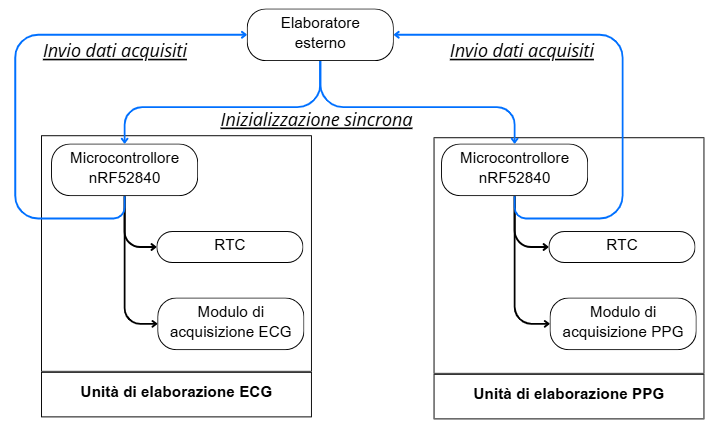
\includegraphics[width=0.8\textwidth]{Schema connessioni}
    \caption{Schema a blocchi dell’architettura delle connessioni hardware del dispositivo wearable. L’elaboratore esterno interagisce con le due unità di acquisizione basate su nRF52840 tramite comunicazione Bluetooth Low Energy (frecce blu), impiegata per la sincronizzazione dei moduli RTC e per la trasmissione dei dati acquisiti. Le connessioni fisiche interne a ciascuna unità, comprendenti collegamenti analogici e digitali cablati (interfaccia I\textsuperscript{2}C/Qwiic) tra microcontrollori e periferiche, sono rappresentate mediante frecce nere.}
    \label{fig:schema_conn}
\end{figure}


\section{Hardware}
L'obiettivo primario del progetto è quello di creare un dispositivo per la stima della pressione cardiaca indossabile basato sul principio del \textit{PAT}, la cui misura necessita dell'acquisizione del segnale elettrocardiografico e del segnale pletismografico lungo un vaso sanguigno arterioso.
Il dispositivo sviluppato è stato progettato con l’obiettivo di acquisire in modo affidabile e sincronizzato segnali fisiologici differenti al fine di consentire analisi combinate e confrontabili nel dominio temporale. Per raggiungere tale obiettivo, l’architettura hardware è stata concepita in maniera modulare, impiegando breakout board commerciali di SparkFun permettendo una rapida integrazione dei componenti e garantendo al contempo buone prestazioni in termini di stabilità e precisione delle misure.
L’acquisizione dei segnali è demandata a due microcontrollori distinti, entrambi basati sul SoC Nordic nRF52840, ciascuno dedicato a una specifica tipologia di segnale. Questa scelta consente di separare le catene di acquisizione, riducendo interferenze e carichi computazionali concorrenti, e migliorando la qualità complessiva dei dati raccolti.
Per garantire un’elevata sincronizzazione temporale tra le due unità di acquisizione, ciascun microcontrollore è stato affiancato da un modulo RTC (Real Time Clock) dedicato, basato sul chip RV-8803. L’uso di orologi in tempo reale ad alta precisione consente di associare timestamp affidabili ai campioni acquisiti, rendendo possibile una successiva analisi sincrona dei segnali ECG e PPG a seguito di una sincronizzazione contemporanea di entrambi gli RTC.
Nei paragrafi seguenti vengono descritti in dettaglio i singoli componenti hardware utilizzati, illustrandone il ruolo all’interno del sistema e le motivazioni che hanno guidato la loro scelta.

\subsection{Microcontrollore nRF52840}
Questo SoC integra un processore ARM Cortex-M4 a 32 bit con unità in virgola mobile (FPU), risultando particolarmente adatto all’elaborazione di segnali fisiologici in tempo reale.
Il nRF52840 è stato scelto principalmente per:
\begin{itemize}
    \item Elevate prestazioni computazionali a fronte di un consumo energetico contenuto, caratteristica fondamentale per dispositivi wearable;
    \item Presenza di un’ampia dotazione di periferiche integrate (ADC, interfacce I²C, BLE);
    \item Compatibilità con ecosistemi di sviluppo consolidati e con le breakboard SparkFun per semplificare la gestione dei sensori e acquisizione segnale.
\end{itemize}
Nel sistema sviluppato, ciascun microcontrollore opera in modo indipendente ed è dedicato all’acquisizione di un solo segnale fisiologico, consentendo una gestione più efficiente delle risorse e una maggiore affidabilità del processo di campionamento.
\begin{figure}[H]
    \centering
    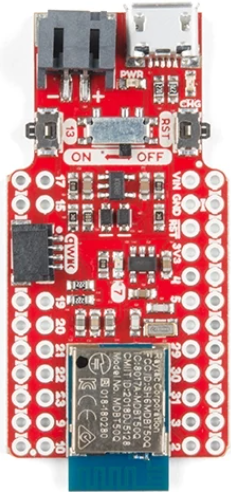
\includegraphics[width=0.15\textwidth]{micro}
    \caption{Rappresentazione del microcontrollore nRF52840}
    \label{fig:micro}
\end{figure}

\subsection{Modulo di acquisizione ECG: AD8232}
Per l’acquisizione del segnale elettrocardiografico è stata utilizzata la breakboard SparkFun basata sul circuito integrato AD8232 di Analog Devices.
L’AD8232 è un front-end analogico specificamente progettato per applicazioni ECG e di monitoraggio biopotenziale, in grado di amplificare e filtrare segnali di ampiezza molto ridotta provenienti dagli elettrodi.
Questo componente integra:
\begin{itemize}
    \item Amplificatore strumentale ad alta precisione;
    \item Stadi di filtraggio configurabili per la riduzione del rumore e degli artefatti di movimento;
    \item Circuiti di rilevamento del contatto degli elettrodi;
    \item Circuiti di pre-processing per calcolo prima derivazione.
\end{itemize}
Nel dispositivo wearable, l’AD8232 svolge il ruolo di condizionamento analogico del segnale ECG prima della digitalizzazione, fornendo in uscita un segnale pulito e compatibile con l’ingresso ADC del microcontrollore nRF52840 dedicato.
\begin{figure}[H]
    \centering
    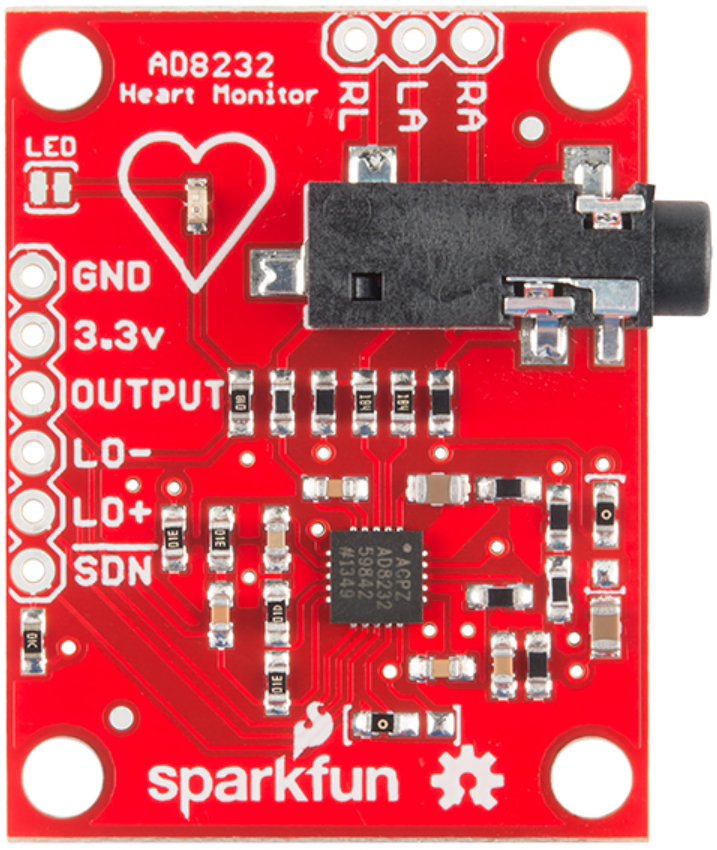
\includegraphics[width=0.15\textwidth]{ECG}
    \caption{Rappresentazione del modulo di acquisizione ECG AD8232}
    \label{fig:ECG}
\end{figure}

\subsection{Modulo di acquisizione PPG: MAX30101 e MAX32664}
Il segnale pletismografico è acquisito tramite la SparkFun Pulse Oximeter and Heart Rate Monitor, una board che integra i dispositivi MAX30101 e MAX32664 di Maxim Integrated.
Il MAX30101 è un sensore ottico che combina LED a diverse lunghezze d’onda e un fotodiodo ad alta sensibilità, permettendo la rilevazione delle variazioni di assorbimento della luce dovute al flusso sanguigno nei tessuti.
Il MAX32664, invece, funge da coprocessore dedicato all’elaborazione dei segnali biometrici, occupandosi della gestione del sensore ottico e dell’estrazione delle informazioni utili dal segnale grezzo.
L’utilizzo di tale board consente di:
\begin{itemize}
    \item Semplificare l’acquisizione del segnale PPG;
    \item Ridurre il carico computazionale sul microcontrollore principale;
    \item Ottenere segnali già pre-elaborati e stabili.
\end{itemize}
Nel sistema sviluppato, il modulo PPG è interfacciato a un secondo microcontrollore nRF52840, dedicato esclusivamente alla gestione di questa catena di acquisizione.
\begin{figure}[H]
    \centering
    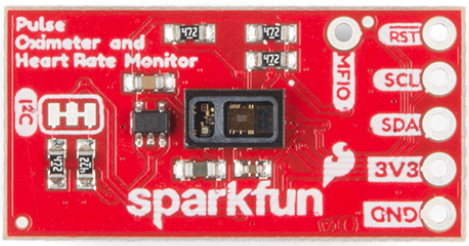
\includegraphics[width=0.15\textwidth]{ppg sensor}
    \caption{Rappresentazione del modulo di acquisizione PPG MAX30101 e sensor-hub MAX32664}
    \label{fig:PPG}
\end{figure}

\subsection{Modulo Real Time Clock: RV-8803}
Per garantire una sincronizzazione temporale accurata tra le due unità di acquisizione, ciascun microcontrollore è affiancato da un Real Time Clock RV-8803 di SparkFun.
Il RV-8803 è un RTC ad alta precisione, caratterizzato da:
\begin{itemize}
    \item Basso consumo energetico;
    \item Elevata stabilità dell’oscillatore;
    \item Interfaccia I²C standardizzata tramite connettore Qwiic.
\end{itemize}
La presenza di un RTC dedicato per ciascun microcontrollore permette di associare un \textit{timestamp} preciso a ogni campione acquisito, rendendo possibile l’allineamento temporale dei segnali ECG e PPG anche in presenza di elaborazioni indipendenti, fondamentale per il contesto applicativo nel quale l'informazione è codificata dalla distanza temporale di fenomeni nei due segnali.
\begin{figure}[H]
    \centering
    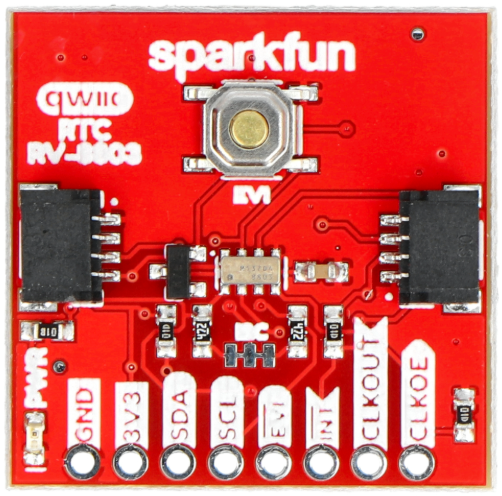
\includegraphics[width=0.15\textwidth]{rtc}
    \caption{Rappresentazione del real time clock RV-8803}
    \label{fig:RTC}
\end{figure}

\section{Alimentazione}
L’alimentazione e la gestione della potenza del dispositivo wearable sono state progettate tenendo conto dei vincoli tipici delle applicazioni indossabili, in cui l’autonomia operativa, la facilità di utilizzo e la manutenibilità rappresentano aspetti fondamentali.
A tal fine, ciascuna delle due unità di acquisizione è alimentata in modo indipendente tramite una batteria dedicata, consentendo un funzionamento autonomo delle due catene hardware e riducendo possibili interdipendenze dal punto di vista energetico.

La scelta di adottare una batteria separata per ciascun dispositivo risulta coerente con l’architettura modulare del sistema e permette una maggiore flessibilità sia in fase di utilizzo sia durante eventuali operazioni di manutenzione. Il contenitore del dispositivo, descritto nella sezione ~\ref{Sezione Case}, è stato progettato in modo da consentire la semplice rimozione e sostituzione della batteria, facilitando l’uso prolungato del sistema senza la necessità di interventi complessi. Inoltre, è prevista la possibilità di ricaricare le batterie collegando direttamente il dispositivo a un computer tramite cavo USB, semplificando le operazioni di ricarica e riducendo la necessità di dispositivi esterni dedicati.

Dal punto di vista dei consumi, il sistema è stato concepito per operare prevalentemente in modalità di minimo consumo, sfruttando le funzionalità di risparmio energetico offerte dai microcontrollori nRF52840 e dai moduli di acquisizione utilizzati. In particolare, le unità di elaborazione sono progettate per limitare l’attività delle periferiche non necessarie e per ridurre il consumo complessivo durante le fasi di inattività o di attesa.

Un aspetto rilevante nella gestione della potenza è rappresentato dalla presenza dei moduli Real Time Clock (RTC), che rimangono alimentati anche in assenza di acquisizione attiva. Per questo motivo, è stato previsto un interruttore hardware che consente di scollegare completamente l’alimentazione del dispositivo, inclusi i moduli RTC. Tale interruttore è sempre accessibile mediante l’apertura del contenitore, permettendo di azzerare i consumi quando il dispositivo non è in uso o durante periodi di inattività prolungata.

Nel complesso, le soluzioni adottate per l’alimentazione e la gestione della potenza rappresentano un compromesso tra autonomia, semplicità di utilizzo e flessibilità del sistema, risultando adeguate alle esigenze di un prototipo wearable orientato all’acquisizione continua di segnali fisiologici.


\section{Connessioni Hardware}
I dispositivi sviluppati presentano differenti tipologie di connessioni hardware, ciascuna adottata in funzione delle specifiche esigenze di acquisizione, comunicazione e gestione dei segnali. In particolare, sono state impiegate:
\begin{itemize}
    \item connessioni analogiche;
    \item connessioni digitali cablate basate sul protocollo Qwiic (I\textsuperscript{2}C);
    \item connessioni wireless Bluetooth Low Energy (BLE).
\end{itemize}

Le diverse tipologie di connessione, rappresentate in Figura~\ref{fig:connessioni}, vengono utilizzate in modo complementare al fine di sfruttare in maniera ottimale le board a disposizione e ottenere un sistema affidabile, modulare e adeguato alle esigenze applicative del dispositivo wearable sviluppato.

\subsection{Connessioni analogiche}
Le connessioni analogiche sono realizzate mediante collegamenti fisici tramite cavi in rame isolato tra i pin analogici delle diverse board. Questo tipo di collegamento consente la trasmissione diretta di segnali analogici al microcontrollore, sia per l’acquisizione di dati provenienti da sensori analogici sia per il controllo di dispositivi di segnalazione, come LED utilizzati per indicare eventuali condizioni di errore.

Nel caso dell’acquisizione dei dati, i segnali analogici vengono instradati verso il convertitore analogico-digitale (ADC) integrato nel microcontrollore nRF52840. L’ADC, di tipo SAR e con risoluzione a 12 bit, viene utilizzato in modalità \emph{single-ended}, in quanto il segnale acquisito non è di tipo differenziale. Questa configurazione consente di ottenere una digitalizzazione del segnale con una risoluzione adeguata, compatibilmente con le frequenze di campionamento richieste per i segnali fisiologici di interesse.

Nel dispositivo sviluppato, le connessioni analogiche sono impiegate principalmente per l’acquisizione del segnale elettrocardiografico. La board utilizzata per l’ECG fornisce infatti un segnale analogico condizionato, senza integrare un’unità di digitalizzazione o di elaborazione digitale, rendendo necessaria l’acquisizione diretta del segnale \emph{raw} da parte del microcontrollore. Inoltre, nello stesso dispositivo, una connessione analogica è utilizzata per il controllo di un LED dedicato alla segnalazione di eventuali errori di connessione degli elettrodi, fornendo un feedback immediato all’utente.

\subsection{Connessioni digitali cablate (Qwiic)}
Ove possibile, si è preferito adottare connessioni digitali cablate al fine di ridurre la complessità del cablaggio e migliorare l’affidabilità complessiva del sistema. In particolare, sono state utilizzate connessioni basate sul protocollo I\textsuperscript{2}C attraverso l’interfaccia Qwiic, che consente di veicolare su un unico collegamento sia l’alimentazione sia i segnali di comunicazione tra il microcontrollore e le periferiche.

Questo tipo di connessione è impiegato in entrambi i dispositivi per la comunicazione tra i microcontrollori nRF52840 e i moduli Real Time Clock (RTC), garantendo una gestione semplice ed efficiente del riferimento temporale. Inoltre, nel dispositivo dedicato all’acquisizione del segnale pletismografico, l’interfaccia Qwiic viene utilizzata per la connessione con il modulo di acquisizione PPG. Tale modulo integra il componente MAX32664, che agisce come \emph{sensor hub}, occupandosi dell’acquisizione digitale del segnale e di una prima fase di pre-elaborazione, riducendo il carico computazionale sul microcontrollore principale.

L’uso delle connessioni Qwiic contribuisce quindi a migliorare la modularità del sistema e a semplificare l’integrazione dei diversi componenti hardware.

\subsection{Connessioni Bluetooth Low Energy (BLE)}
Le connessioni \textit{Bluetooth Low Energy (BLE)} sono utilizzate esclusivamente per la comunicazione wireless tra i dispositivi wearable e un elaboratore esterno, che funge da nodo di controllo e raccolta dei dati. In questa configurazione, il computer opera come master della connessione, mentre i dispositivi wearable agiscono come nodi periferici.

La comunicazione \textit{BLE} viene impiegata in due contesti principali. Il primo riguarda l’invio, da parte del computer, del comando di sincronizzazione temporale, utilizzato per allineare i moduli RTC associati ai due microcontrollori e garantire una base temporale comune per l’acquisizione dei segnali. Il secondo contesto riguarda la trasmissione dei dati acquisiti dai dispositivi verso il computer. Tale trasmissione avviene in modo alternato tra le due unità, al fine di evitare conflitti sul canale di comunicazione e consentire un’analisi dei segnali in tempo reale o semi-real time.

L’adozione della comunicazione BLE permette di eliminare collegamenti fisici diretti con l’elaboratore esterno, aumentando la flessibilità del sistema e rendendo il dispositivo più adatto a un utilizzo in ambito wearable.
\begin{figure}[H]
    \centering
    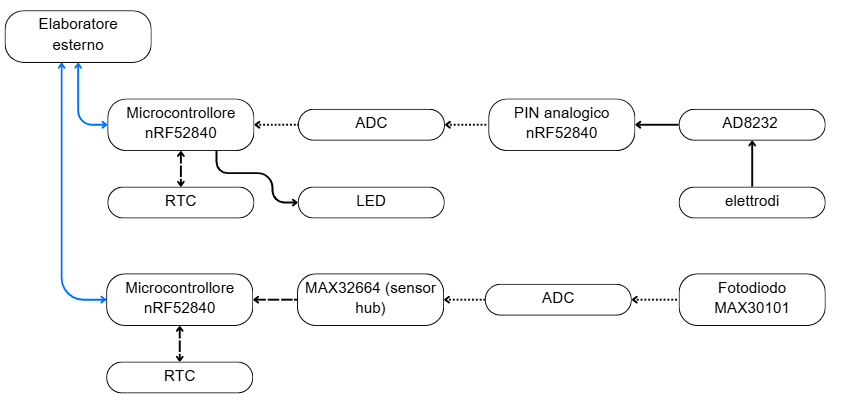
\includegraphics[width=0.8\textwidth]{immagine capitolo 4}
    \caption{Schema a blocchi delle connessioni hardware del dispositivo wearable sviluppato. Le frecce blu indicano le comunicazioni wireless \textit{BLE} tra le due unità di acquisizione e l’elaboratore esterno, utilizzate per la sincronizzazione dei moduli RTC e per la trasmissione dei dati acquisiti. Le connessioni fisiche interne alle unità sono rappresentate in nero: linee continue per i collegamenti analogici, linee tratteggiate per i bus digitali Qwiic/I²C, e linee a puntini per le connessioni tra componenti già integrati sulla stessa board. Questa rappresentazione permette di visualizzare i percorsi reali dei segnali, evidenziando i diversi tipi di collegamento utilizzati all’interno del sistema.
}
    \label{fig:connessioni}
\end{figure}

\subsection{Schematici}
La strategia adottata per la realizzazione dell'hardware prevede l'uso di una \textit{Baseboard} progettata ad hoc. Questa scheda funge da interfaccia di collegamento, ospitando connettori femmina (header) destinati ad accogliere le breakout board dei vari componenti (Microcontrollore, RTC, Sensori). Tale approccio garantisce una stabilità meccanica e un'affidabilità elettrica nettamente superiori rispetto alla prototipazione su breadboard o millefori, eliminando le incertezze dovute a saldature volatili o collegamenti tramite jumper wires, pur mantenendo la modularità necessaria in fase di prototipazione.
La stesura degli schematici per le due unità (ECG e PPG) ha seguito un rigoroso flusso di progettazione volto a garantire la corretta corrispondenza tra il componente fisico e la sua rappresentazione CAD. Il processo ha previsto:
\begin{itemize}
    \item L'analisi dei datasheet forniti dai produttori \cite{sparkfun_nrf52840}\cite{sparkfun_ppg_sensor}\cite{sparkfun_rv8803}\cite{sparkfun_ad8232} per identificare piedinature e specifiche elettriche.
    \item La creazione delle librerie CAD (in ambiente Eagle), con particolare attenzione alla definizione delle \textit{footprint} corrette per i connettori.
    \item L'integrazione logica dei componenti, verificando le connessioni di alimentazione, i bus di comunicazione (I2C) e le linee di interrupt.
\end{itemize}

\begin{figure}[H]
    \centering
    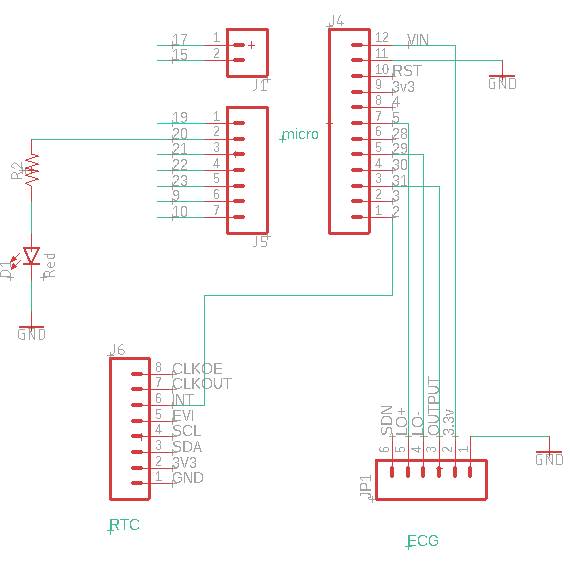
\includegraphics[width=0.5\textwidth]{schematico ECG}
    \caption{Schematico ECG: Contiene due file di connettori relativi al microcontrollore, connettori RTC, connettori modulo ECG e un LED con la relativa resistenza.}
\end{figure}

\begin{figure}[H]
    \centering
    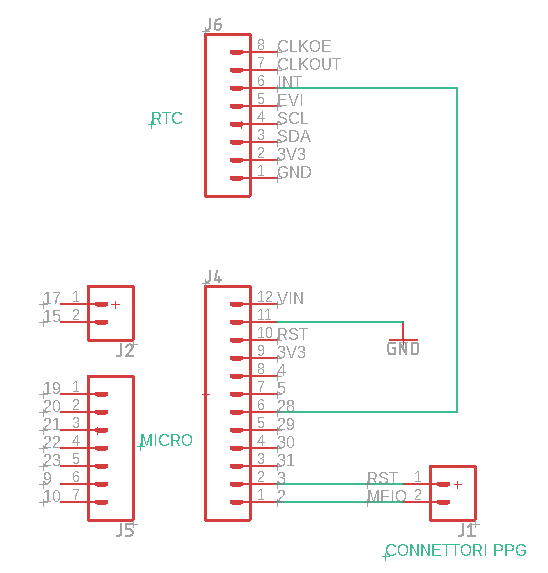
\includegraphics[width=0.5\textwidth]{schematico PPG}
    \caption{Schematico PPG: Contiene due file di connettori relativi al microcontrollore e connettori RTC. I collegamenti risultano essere pochié la quasi totalità dei dati è trasmessa tramite i cavi QWIIC.}
\end{figure}

\subsection{PCB}
Il layout del Circuito Stampato (PCB) per l'unità ECG è stato ottimizzato per ricalcare gli ingombri del prototipo iniziale, riservando un'area dedicata all'alloggiamento della batteria.
Nel layer serigrafico (\textit{Silkscreen}), sono state riportate le sagome delle breakout board per facilitare il corretto orientamento e montaggio dei moduli durante la fase di assemblaggio.

Dal punto di vista dell'integrità del segnale, sono stati adottati i seguenti accorgimenti progettuali:
\begin{itemize}
    \item \textbf{Piani di Massa (Ground Planes):} Sia sul Top che sul Bottom layer è stata applicata una \textit{Copper Pour} connessa a massa (GND) per minimizzare i disturbi elettromagnetici e fornire un riferimento stabile.
    \item \textbf{Layout RF e Keep-out Zone:} In corrispondenza dell'antenna integrata nel modulo nRF52840, è stata definita un'area di \textit{Keep-out} priva di piste in rame e piani di massa. Sebbene le linee guida suggeriscano di posizionare l’antenna esternamente al perimetro della PCB, i test empirici sul prototipo non hanno evidenziato interferenze significative del segnale BLE con la configurazione attuale: ciò ha permesso così di ottimizzare la compattezza del dispositivo.
\end{itemize}

\begin{figure}[H]
    \centering
    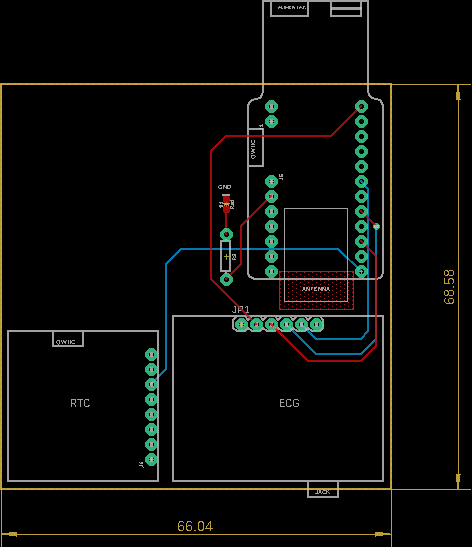
\includegraphics[width=0.5\textwidth]{PCB ECG}
    \caption{PCB ECG}
\end{figure}

\begin{figure}[H]
    \centering
    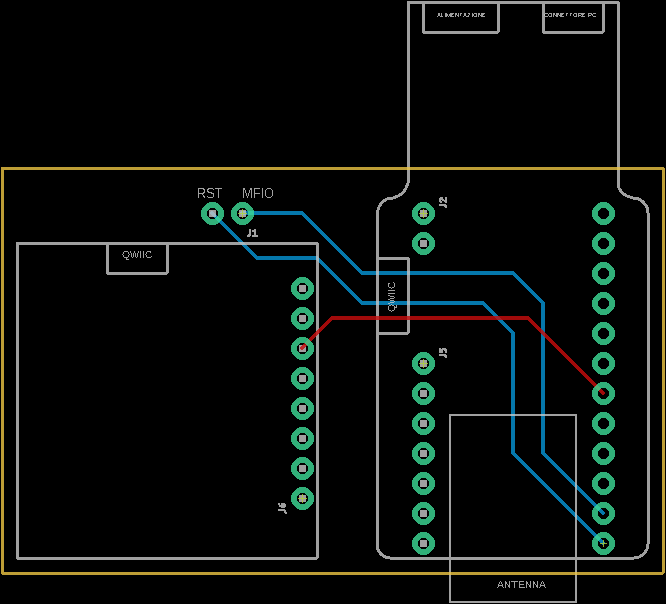
\includegraphics[width=0.5\textwidth]{PCB PPG 3.png}
    \caption{PCB PPG}
\end{figure}

\section{Architettura Firmware e Logica di Acquisizione}
Il firmware sviluppato per le unità di acquisizione (ECG e PPG) è stato progettato con l'obiettivo primario di garantire un determinismo temporale rigoroso, condizione necessaria per la successiva analisi del PAT. L'architettura sfrutta un approccio event-driven gestito tramite interrupt hardware, delegando la scansione temporale a un componente esterno ad alta precisione (RTC) piuttosto che ai timer interni del processore, spesso soggetti a jitter dovuti alla gestione dello stack Bluetooth.

Di seguito vengono descritti i moduli funzionali che compongono il firmware.
\subsection{Gestione della Connessione Bluetooth Low Energy (BLE)}
\label{sec:BLE}
Il sistema opera in una topologia di tipo Piconet, dove il PC agisce da \textit{Central Master} e le due board di acquisizione agiscono da Peripherals (\textit{Slaves}). All'avvio, il firmware inizializza lo stack BLE configurando il dispositivo in modalità di rilevamento generale (\textit{General Discovery Mode}) per consentire al master di individuare il sensore all'interno della piconet senza restrizioni temporali. Per massimizzare la quantità di dati inviati e ridurre la latenza, sono stati ottimizzati due parametri critici:
\begin{itemize}
    \item \textit{Connection Interval}: È stato impostato un intervallo di connessione ridotto (tra 7.5 ms e 15 ms), permettendo scambi di dati frequenti.
    \item \textit{MTU (Maximum Transmission Unit)}: La larghezza di banda è stata massimizzata negoziando una dimensione del pacchetto superiore allo standard.
\end{itemize}
Per garantire la robustezza del sistema, è stata implementata una Callback di Disconnessione. Questo meccanismo di sicurezza monitora costantemente lo stato del link radio: in caso di perdita di segnale o chiusura forzata del software lato PC, il firmware intercetta l'evento, interrompe immediatamente l'acquisizione e pone i sensori in stato di idle, disabilitando gli interrupt per prevenire consumi energetici inutili o errori di stato alla riconnessione successiva.

\subsection{Sincronizzazione e Protocollo di Start}
Uno degli aspetti più critici del progetto è la sincronizzazione temporale tra le due unità indipendenti. Poiché non esiste un collegamento fisico tra le board, la sincronizzazione avviene via software tramite un comando broadcast.

Il firmware implementa una macchina a stati finiti, il cui diagramma di flusso completo è raffigurato in figura \ref{fig:workflow firmware}. All'accensione, il sistema entra in uno stato di "Attesa". L'acquisizione vera e propria inizia solo alla ricezione di un carattere specifico sulla seriale BLE. La ricezione di questo comando innesca una procedura "atomica" (non interrompibile) che esegue tre azioni in sequenza immediata:
\begin{enumerate}
  \item Reset dei Contatori: Il contatore globale dei tick (timestamp) viene azzerato.
  \item Configurazione Buffer: Vengono preparati i puntatori alla memoria per il primo pacchetto dati.
  \item Abilitazione RTC: Viene inviato il comando I2C all'RTC per iniziare il conteggio hardware.
\end{enumerate}

Questa procedura garantisce che l'errore di allineamento temporale tra le due board sia limitato alla sola latenza di propagazione del segnale Bluetooth (nell'ordine dei millisecondi) e alla gestione dell'interrupt, risultando trascurabile per le dinamiche fisiologiche osservate.

\subsection{Generazione del Time-Base tramite Interrupt Hardware (RTC)}
Per svincolare il microcontrollore dal compito oneroso di mantenere il tempo mentre gestisce la comunicazione radio, è stato utilizzato un Real-Time Clock (RTC) esterno configurato in modalità Periodic Countdown Timer.

Invece di interrogare l'RTC via I2C per ottenere l'orario a ogni campione (operazione che introdurrebbe latenze non deterministiche dovute al bus I2C), il firmware configura l'RTC per generare un segnale elettrico (onda quadra) su un pin fisico collegato al microcontrollore.
\begin{itemize}
  \item Per la board PPG: L'RTC è programmato per generare un interrupt a 256 Hz.
  \item Per la board ECG: Data la necessità di catturare la morfologia rapida del complesso QRS, la frequenza è raddoppiata a 512 Hz.
\end{itemize}
Ogni volta che l'RTC genera un impulso, scatta una Interrupt Service Routine (ISR) ad altissima priorità. Questa funzione è volutamente minimale per non bloccare il processore: si limita a incrementare il contatore globale dei campioni e ad alzare un flag di "richiesta campionamento". Questo approccio garantisce che il jitter di campionamento sia virtualmente nullo.

\subsection{Acquisizione e Double Buffering}
Il loop principale del firmware gestisce l'acquisizione vera e propria. Quando il flag di interrupt viene rilevato, il processore esegue la lettura del sensore:
\begin{itemize}
    \item \textbf{ECG:} Viene effettuata una lettura analogica (ADC) del segnale condizionato dall'AD8232.
    \item \textbf{PPG:} Viene interrogato via I2C il sensore bio-hub per ottenere il valore grezzo del LED infrarosso.
\end{itemize}

Per gestire il flusso continuo di dati senza perdite durante la trasmissione Bluetooth (che può richiedere diversi millisecondi), è stata implementata una logica di \textit{Double Buffering}. Sono stati allocati due array di memoria identici, denominati \texttt{Buffer A} e \texttt{Buffer B}. Il funzionamento è il seguente:
\begin{enumerate}
    \item Il sistema scrive i nuovi campioni nel \texttt{Buffer A}.
    \item Appena il \texttt{Buffer A} è pieno (raggiunto il numero di campioni pari a 1 secondo di acquisizione), il sistema commuta istantaneamente la scrittura sul \texttt{Buffer B}.
    \item Contemporaneamente, il \texttt{Buffer A} viene "congelato" e passato alla routine di trasmissione BLE.
\end{enumerate}
Questo meccanismo permette di trasmettere i dati del secondo precedente mentre si acquisiscono quelli del secondo corrente, garantendo continuità assoluta nel segnale registrato.

\begin{figure}[H]
    \centering
    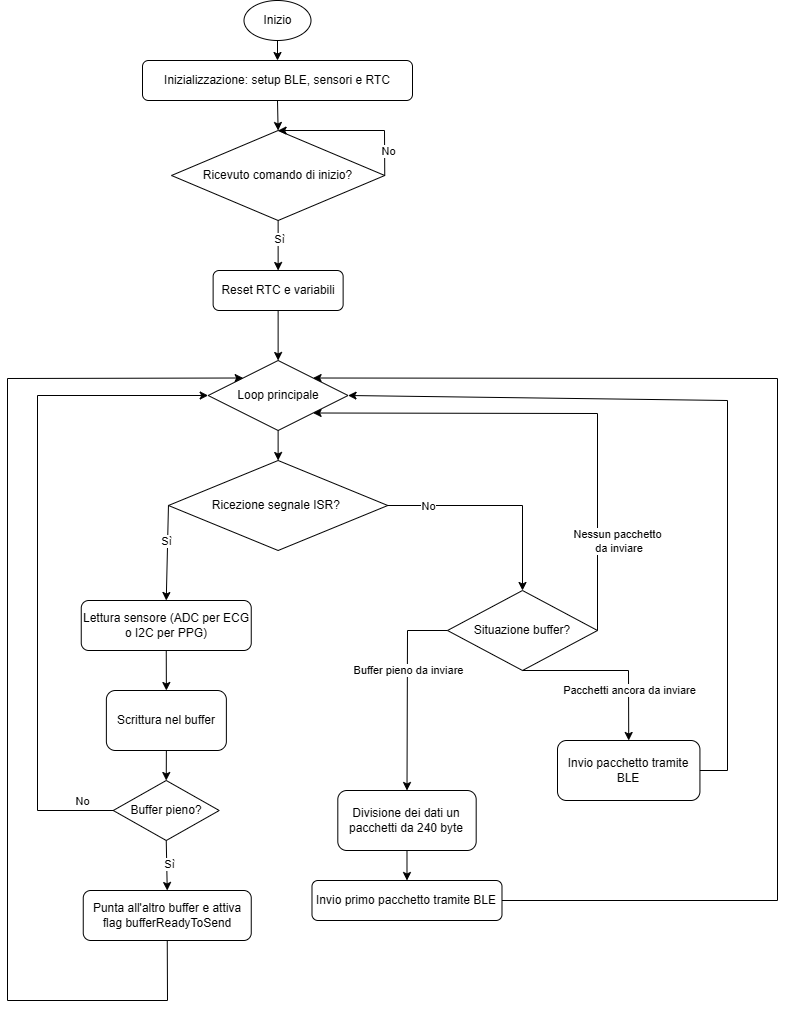
\includegraphics[width=0.8\textwidth]{Diagramma flusso PAT.drawio}
    \caption{Diagramma di flusso firmware}
    \label{fig:workflow firmware}
\end{figure}

\subsection{Strategia di Trasmissione}
La trasmissione dei dati via BLE rappresenta il potenziale collo di bottiglia del sistema. Per evitare la saturazione del canale e la perdita di pacchetti, sono state adottate due strategie fondamentali:

\textbf{A. Frammentazione e Overhead Reduction:} Invece di inviare ogni singolo campione individualmente (che comporterebbe un enorme overhead protocollare), i dati vengono accumulati e inviati in blocchi. Quando un buffer è pronto per l'invio, il firmware costruisce un macro-pacchetto contenente:
\begin{itemize}
    \item Un Header di 4 byte con il \texttt{timestamp} (il numero di tick) dell'inizio del blocco.
    \item Il Payload contenente i campioni a 16 bit.
\end{itemize}
Questo macro-pacchetto viene poi frammentato e inviato in micro-pacchetti di 240 byte. Questa dimensione non è casuale, ma è calibrata per sfruttare al massimo la \textit{Data Length Extension} del Bluetooth 5.0, riducendo drasticamente il numero di transazioni radio necessarie per trasferire un secondo di dati rispetto ai pacchetti standard da 20 byte.


\textbf{B. Sfasamento Temporale:} Per prevenire collisioni radio nel caso in cui entrambe le schede tentino di trasmettere un pacchetto voluminoso nel medesimo istante, è stato introdotto uno sfasamento intenzionale nella logica di riempimento dei buffer.
\begin{itemize}
    \item La board ECG riempie buffer da 1 secondo intero (512 campioni).
    \item La board PPG, solo per il primo ciclo di acquisizione, riempie un buffer ridotto di 0.5 secondi (128 campioni), per poi passare a buffer standard da 1 secondo (256 campioni).
\end{itemize}
In questo modo, le trasmissioni delle due board risultano alternarsi: quando una trasmette, l'altra è circa a metà del riempimento del proprio buffer. Questo riduce la congestione sul ricevitore (PC) e migliora la stabilità del link.
    



\section{Software di Ricezione ed Elaborazione dei dati}

La ricezione dei dati e la loro elaborazione vengono gestiti tramite un software sviluppato in linguaggio Python, sfruttando la libreria \texttt{asyncio} (per comunicazioni asincrone). Il programma gestisce la comunicazione contemporanea con i due dispositivi BLE e l'elaborazione del segnale in tempo reale, definendo il PC come \textit{Master} e le board come \textit{Slaves}, come detto nella sezione \ref{sec:BLE}. Il sistema deve quindi occuparsi nell'ordine della gestione della comunicazione, del buffering dei dati, degli algoritmi di signal processing e del salvataggio dei dati predisposti all'interfaccia.

\subsection{Ricezione dei Dati}

Il modulo di ricezione è specifico per la strategia di comunicazione adottata nel firmware. La comunicazione si basa quindi sul protocollo BLE e viene gestita tramite la libreria Python \texttt{Bleak}, che configura il PC come \textit{GATT Client (Generic Attribute Profile)}. 

Non si tratta dunque di un approccio di tipo \textit{polling}, che avrebbe inevitabilmente aumentato la latenza di ricezione e l'occupazione della banda radio, quanto di un'architettura basata su delle Notifiche. All'inizio del programma, il \textit{client} effettua la sottoscrizione alla caratteristica UART TX, ponendosi in ascolto passivo: solo quando i buffer di trasmissione sono pronti, le board li inviano.

Per gestire simultaneamente i due flussi dati asincroni, il software istanzia due oggetti handler distinti (uno per ECG e uno per PPG). Ciascun handler instaura una connessione dedicata e identifica la periferica target analizzando il \textit{Local Name} esposto durante la fase di \textit{advertising}:
\begin{itemize}
    \item L'handler per l'ECG si connette esclusivamente al dispositivo identificato come "boardECG".
    \item Quello per la PPG si connette esclusivamente al dispositivo identificato come "boardPPG".
\end{itemize}

Questo permette di parallelizzare la ricezione dei pacchetti, indirizzando i dati grezzi verso le rispettive routine di decodifica. Il flusso logico di ricezione è il seguente: 

\begin{itemize}
    \item \textbf{Decoding del pacchetto}: Il software discrimina automaticamente la tipologia di pacchetto arrivato basandosi sulla dimensione in byte e ricostruendo la base temporale corretta. Se la lunghezza è di 4 byte, il pacchetto viene interpretato come Header di sincronizzazione (\texttt{timestamp}); qualsiasi altra dimensione viene interpretata come Payload contenente i campioni del segnale. Quindi, in particolare:
    \begin{itemize}
        \item Header (4 byte): Identifica l'inizio di un nuovo blocco dati, decodificato come intero a 32-bit che rappresenta il \texttt{timestamp} assoluto al momento di generazione del blocco.
        \item 
        Payload: Contiene la sequenza dei campioni fisiologici, decodificato come una serie di interi a 16-bit corrispondenti ai valori grezzi dell'ADC.
    \end{itemize}
    \item \textbf{Buffering}: I dati ricevuti vengono accodati in due rispettivi buffer circolari e parallelamente scritti su due file CSV (\texttt{ecg\_[timestamp].csv} e \texttt{ppg\_[timestamp].csv}).
\end{itemize}

\subsection{Elaborazione dei Dati}
L'elaborazione dei dati appartenti ai buffer avviene su finestre temporali per permettere l'applicazione stabile di filtri digitali. Questo viene implementato usando una finestra mobile di 6 secondi che avanza di 1 secondo alla volta, con una sovrapposizione di 5 secondi.
Il main loop esegue la routine di analisi con una periodicità di 1 secondo. Ad ogni ciclo di analisi, l'algoritmo preleva dal buffer gli ultimi 6 secondi di segnale: questa sovrapposizione evita effetti di bordo dei filtri e garantisce che nessun picco venga perso. Una volta estratti i punti fiduciali necessari, il sistema calcola il PAT accoppiando ogni picco R con il primo piede PPG successivo. L'evento, ovvero l'accoppiamento, viene considerato valido unicamente quando la differenza temporale è inferiore a 1500 ms. Contestualmente, viene calcolata la frequenza cardiaca istantanea basata sull'intervallo RR tra gli ultimi due picchi ECG rilevati.

\subsubsection{Algoritmo di individuazione dei picchi ECG}
Per l'individuazione del picco R è stato adottato l'algoritmo di Pan-Tompkins, il che risulta essere quello tutt'ora più utilizzato in letteratura \cite{mukkamala2015}. Ne è stata implementata una versione leggermente modificata, adeguandone i parametri al nostro sistema d'acquisizione e alla finestra di tempo considerata. 

Sono previste le quattro tradizionali fasi:
\begin{enumerate}
    \item Filtro Passa-Banda: il segnale grezzo viene filtrato con un filtro Butterworth del primo ordine con banda passante 5-15 Hz per rimuovere la deriva della baseline e i rumori di rete/muscolari.
    \item Enfatizzazione complesso QRS: si calcola la differenza tra campioni adiacenti (derivata) per evidenziare le pendenze elevate. Questo passaggio risulta essere una versione semplificata a 2 punti rispetto al derivatore a 5 punti dello schema classico. Dopodiché, si eleva al quadrato il segnale così derivato per rendere positivi tutti i dati ed enfatizzare le alte frequenze; infine, viene applicata una integrazione con una finestra mobile di 150 ms per ottenere l'inviluppo dell'energia del segnale.
    \item Rilevamento picchi: sull'inviluppo integrato viene applicata la funzione \textit{find\_peaks}, con una soglia adattativa pari a 2 volte la media del segnale integrato nella finestra corrente. A differenza dell'approccio originale, che utilizza un sistema di soglie adattive con memoria storica aggiornate di battito in battito, questo metodo ricalcola la soglia staticamente per ogni finestra di analisi, ottimizzando il processo per l'elaborazione a buffer. Per quanto riguarda i parametri, viene impostata una distanza minima tra i picchi di 250 ms (periodo refrattario fisiologico) per evitare di rilevare l'onda T o altri artefatti come falsi positivi. 
    \item Ricerca picco sul segnale: una volta individuata la posizione approssimativa del picco R, si cerca il massimo assoluto sul segnale grezzo originale in un intorno di ±100 ms, per garantire un'adeguata precisione temporale e compensare lo sfasamento temporale introdotto dalla precedente integrazione.
\end{enumerate}

\subsubsection{Algoritmo di individuazione dei piedi PPG}

L'individuazione dell'onset sistolico (o piede dell'onda PPG) è preferibile all'individuazione di un qualsiasi altro punto fiduciale sull'onda poiché molto più riproducibile \cite{mukkamala2015}. In letteratura, i metodi per rilevarlo sono molteplici come, per citarne alcuni, il metodo delle tangenti (giudicato il più robusto) \cite{mukkamala2015}, metodi basati su cross-correlazione con altri segnali PPG provenienti da diversi punti \cite{lazazzera2019} o sul calcolo della derivata \cite{Welykholowa2020-pu} o ancora, più semplicemente, soglie adattative sul minimo assoluto \cite{Finnegan2021} . La scelta di collocare il sensore PPG sul piede \cite{Block2020-ad}, ha reso troppo rumoroso e quindi complicato l'utilizzo di alcuni di questi algoritmi riconosciuti. Dunque, dopo aver provato inefficacemente con altre metodologie, si è optato per l'attuazione di un algoritmo custom che prevede la rilevazione del minimo relativo alla specifica finestra temporale. Questo segue i seguenti passaggi: 
\begin{enumerate}
  \item Rimozione della Baseline: In letteratura si concorda che risulta necessario pre-filtrare il segnale nella banda di interesse per la rilevazione di questo punto nell'onda PPG [0.5 - 5 Hz]. Viene quindi sottratta la componente continua calcolata tramite una media mobile centrata con finestra di 0.75 secondi.
  \item Filtraggio Passa-Basso: Si applica un filtro Butterworth del 4° ordine con frequenza di taglio a 5 Hz per eliminare il rumore ad alta frequenza e l'onda dicrota (che potrebbe essere confusa con un piede), mantenendo solo le armoniche fondamentali dell'onda sfigmica.
  \item Normalizzazione (Z-Score): Per rendere l'algoritmo robusto rispetto alle variazioni di ampiezza del segnale (dovute a movimenti o vasocostrizione), viene calcolato lo Z-Score locale la cui deviazione standard è calcolata su una finestra mobile di 2 secondi.
  \item Rilevamento Piedi: Poiché l'interesse è sui minimi locali (piedi), il segnale Z-Score viene invertito. Si cercano i picchi sul segnale invertito con i seguenti parametri restringenti derivati da prove effettuate con il sistema d'acquisizione disponibile:
\begin{itemize}
    \item Prominenza: 0.6 (per distinguere il picco dal rumore)
\item Altezza minima: 0.9 (soglia dello Z-Score)
\item Distanza minima: 400 ms (per evitare doppi rilevamenti)
\end{itemize}
\end{enumerate}

\subsection{Struttura dei Dati Salvati}
Il salvataggio dei dati avviene attraverso un database relazionale SQL, progettato per garantire coerenza, tracciabilità e integrazione diretta con l’interfaccia grafica e con i moduli di elaborazione dei segnali.

Ogni sessione di acquisizione è identificata univocamente all’interno della tabella \texttt{misure}, che rappresenta l’elemento centrale del modello dati. In essa vengono memorizzate le informazioni contestuali della misura, tra cui il periodo della giornata (mattina, pomeriggio o sera), la data di acquisizione, il riferimento alla calibrazione utilizzata (tra quelle salvate selezionabili, nella tabella \texttt{calibrazioni}, ad esempio con un unico dispositivo e un unico account potrei voler misurare la pressione di più persone all'interno di un nucleo familiare) e l’utente che ha effettuato la misurazione. Tutti i dati grezzi ed elaborati risultano logicamente collegati a questa entità tramite chiavi esterne.

Il salvataggio dei dati è organizzato su due livelli concettualmente distinti: un livello di dati grezzi e un livello di dati elaborati.

\subsubsection{Dati Grezzi}
I campioni grezzi acquisiti relativi ai segnali ECG e PPG vengono memorizzati all’interno della tabella \texttt{campioni}. Ogni record rappresenta un singolo campione e contiene il tipo di segnale (ECG o PPG), l’ampiezza misurata, il timestamp di acquisizione e il riferimento all'entità della tabella \texttt{misure} a cui il campione appartiene.

La scrittura dei dati avviene in tempo reale all’interno della routine di gestione delle notifiche BLE: ogni pacchetto ricevuto dal microcontrollore viene decodificato e i campioni risultanti vengono immediatamente inseriti nel database. Questa modalità consente di preservare l’ordine temporale e l’integrità del segnale originale, rendendo possibile una ricostruzione fedele dell’andamento dei segnali acquisiti.

Le informazioni relative a diversi eventuali dispositivi utilizzabili per le acquisizioni sono memorizzate nella tabella \texttt{dispositivi}. Essa descrive, per ciascun dispositivo, il nome, il tipo di segnale misurato e un eventuale riferimento a materiale descrittivo o fotografico. Questo approccio consentirebbe in futuro di disaccoppiare i dati di misura dalle caratteristiche hardware.

\subsubsection{Risultati dell’Elaborazione}
I risultati prodotti dagli algoritmi di elaborazione dei segnali (picchi R del segnale ECG e piedi dell'onda del segnale PPG) vengono inizialmente salvati in variabili temporanee per estrarre PAT e HR; tali dati vengono quindi utilizzati per la stima della pressione, che viene memorizzata nella tabella \texttt{indici\_misura}.

Per ciascun intervallo di analisi vengono salvati i \texttt{timestamp} di riferimento e i valori calcolati. Come detto in precedenza, ogni evento di misurazione permette di selezionare una calibrazione. Il processo di elaborazione si basa quindi sui parametri della calibrazione selezionata, memorizzati nella tabella \texttt{calibrazioni}, che contiene i coefficienti corrispondenti. Questo consente di adattare i modelli di stima alle caratteristiche del singolo utente o dispositivo, determinando l’accuratezza delle misure derivate.

Infine, le informazioni anagrafiche e biometriche dell’utente sono gestite nella tabella \texttt{users}, che permette di collegare ogni misura a un profilo specifico, garantendo la coerenza tra dati fisiologici, parametri personali e risultati dell’elaborazione.



\section{Software di Interfaccia utente}
Al fine di garantire la massima usabilità del dispositivo sviluppato, è stato concepito un ambiente digitale integrato che permette all’utente di interagire con tutte le funzionalità del sistema in modo semplice e immediato. L’applicazione, in Figura~\ref{fig:foto_app}, non si limita alla semplice visualizzazione dei dati raccolti dai sensori, ma rappresenta un vero e proprio portale completo per la gestione del monitoraggio della salute, dove l’utente può sia acquisire nuove misure che consultare i dati precedentemente registrati, aggiornare le proprie informazioni personali e accedere a risorse informative e di supporto.
L’obiettivo principale della progettazione dell’interfaccia è stato quello di creare un ambiente flessibile e scalabile, in grado di supportare non solo il dispositivo attualmente sviluppato, ma anche eventuali futuri sensori o dispositivi aggiuntivi. Questa architettura permette di integrare facilmente nuovi parametri fisiologici e funzionalità, senza richiedere modifiche sostanziali all’infrastruttura esistente, garantendo così una continuità d’uso e la possibilità di evolvere nel tempo insieme alle esigenze degli utenti.
\begin{figure}
    \centering
    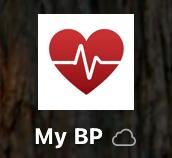
\includegraphics[width=0.2\linewidth]{Images/foto_app.jpeg}
    \caption{Logo applicazione}
    \label{fig:foto_app}
\end{figure}


Ogni individuo che utilizza il dispositivo dispone di un account personale, attraverso il quale può gestire in modo completo tutte le informazioni relative alla propria salute. Una volta effettuato l’accesso, l’utente ha la possibilità di svolgere una serie di attività fondamentali per il monitoraggio quotidiano:
\begin{itemize}
    \item \textbf{Login e registrazione}: accesso o creazione di un profilo per un utente.
    \item \textbf{Acquisizione di nuove misure}: avvio e gestione del processo di registrazione dei dati fisiologici tramite i dispositivi indossabili, con possibilità di visualizzare in tempo reale i segnali raccolti e monitorarne l’andamento.
    \item \textbf{Consultazione dello storico dei dati}: accesso alle misure precedentemente registrate, con opzioni per visualizzare singole sessioni o statistiche aggregate, filtrare le informazioni per intervallo temporale e analizzare l’evoluzione di parametri come pressione arteriosa, frequenza cardiaca e segnali ECG/PPG.
    \item \textbf{Gestione del profilo utente}: aggiornamento dei dati personali, caricamento o modifica dell’immagine del profilo, inserimento e aggiornamento di peso, altezza e numeri di contatto, oltre alla possibilità di cambiare la password per garantire la sicurezza dell’account.
    \item \textbf{Accesso a risorse informative}: consultazione di domande frequenti (\textit{FAQ}) e materiale informativo relativo alla salute cardiovascolare, al corretto utilizzo del dispositivo e alla lettura dei dati, così da supportare l’utente sia dal punto di vista pratico che educativo.
    \item \textbf{Supporto tecnico}: contatto diretto con il team di assistenza in caso di problemi o dubbi sull’utilizzo dell’applicazione o del dispositivo.
    \item \textbf{Logout sicuro}: possibilità di chiudere la sessione in maniera protetta, evitando accessi non autorizzati e preservando la privacy dei dati personali.
\end{itemize}

Per facilitare la navigazione e garantire un accesso rapido a tutte le sezioni principali, è stato implementato un menù laterale comprimibile, posizionato sul lato sinistro dell’interfaccia. Questo elemento permette all’utente di avere sempre sotto controllo le funzionalità disponibili senza sacrificare spazio prezioso per la visualizzazione dei dati e dei grafici, mantenendo l’interfaccia ordinata e intuitiva. Come mostrato in Figura~\ref{fig:foto1}, il menù fornisce un accesso immediato alle diverse sezioni, favorendo un’esperienza utente fluida e coerente.
\begin{figure}[H]
    \centering
    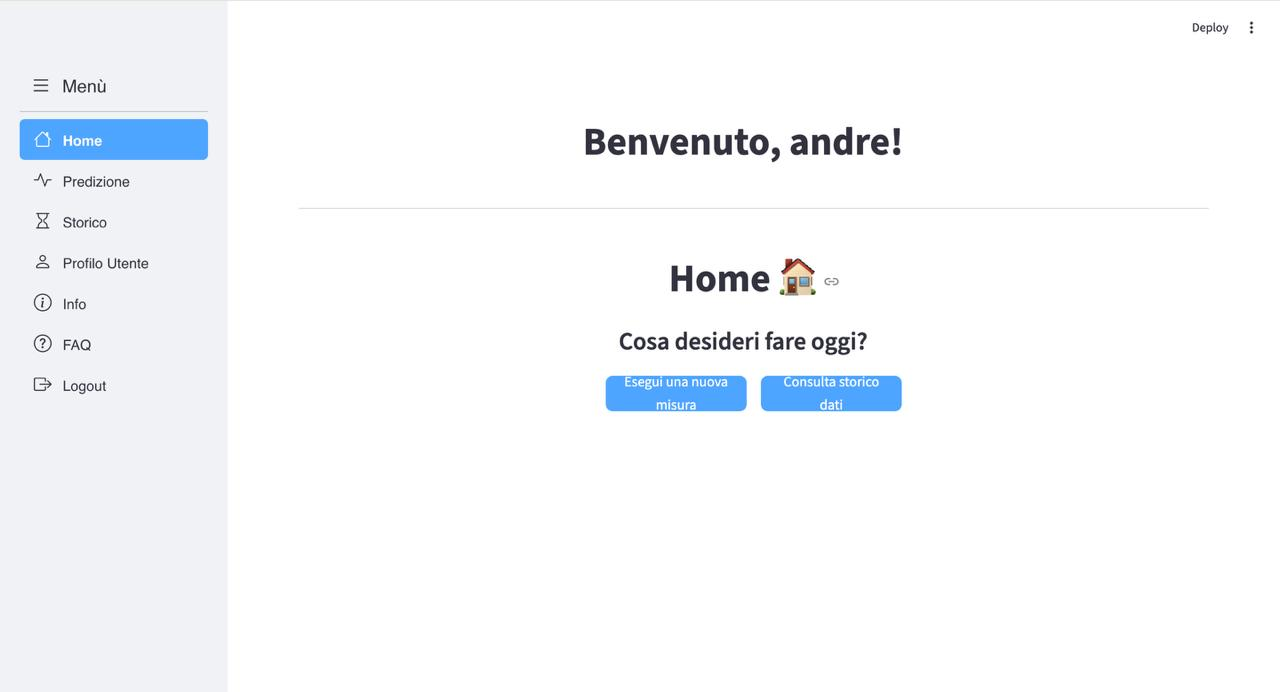
\includegraphics[width=1\linewidth]{Images/elenco laterale.jpeg}
    \caption{Menù laterale comprimibile, accesso rapido alle principali funzionalità.}
    \label{fig:foto1}
\end{figure}
A seguire vengono presentate in dettaglio le singole pagine dell’interfaccia, con la descrizione delle funzionalità offerte, dei contenuti visualizzati e delle modalità di interazione disponibili. Ogni sezione è strutturata per illustrare chiaramente come l’utente può accedere ai dati, interpretare le informazioni e gestire le proprie impostazioni, offrendo una panoramica completa del sistema e della sua esperienza d’uso.

\subsection{Login e registrazione}
La pagina di Login rappresenta il punto di accesso principale all’applicazione ed è stata progettata per garantire un’interazione chiara, intuitiva e guidata fin dal primo utilizzo. Attraverso questa schermata, l’utente può autenticarsi al sistema oppure creare un nuovo account personale, necessario per accedere a tutte le funzionalità di monitoraggio offerte dalla piattaforma. In una prima fase vengono presentati due pulsanti principali, che consentono di scegliere tra la procedura di registrazione e quella di accesso. Questa separazione permette di mantenere l’interfaccia ordinata e di mostrare solo le informazioni rilevanti in base all’azione selezionata.
\begin{itemize}
\item Nel caso di registrazione, all’utente viene richiesto di inserire una serie di dati personali e biometrici, tra cui informazioni anagrafiche, parametri fisici e recapiti telefonici, inclusi i contatti di emergenza. La procedura è accompagnata da controlli di validazione che verificano la correttezza dei dati inseriti, garantendo l’integrità delle informazioni memorizzate nel sistema. Al termine della registrazione, l’utente riceve una conferma visiva dell’avvenuta creazione dell’account.
\item La procedura di login consente invece agli utenti già registrati di accedere all’applicazione tramite l’inserimento delle proprie credenziali. Il sistema verifica l’autenticità dei dati forniti e, in caso di esito positivo, inizializza la sessione utente, permettendo l’accesso alle funzionalità principali dell’applicazione. 
\end{itemize}
In caso di errore, vengono forniti messaggi chiari e immediati per facilitare la risoluzione del problema.

\subsection{Acquisizione nuova misura}
La sezione di acquisizione di una nuova misura permette di eseguire tutti i passaggi necessari al fine di personalizzare le caratteristiche della misura, gli strumenti da utilizzare e le eventuali calibrazioni.
In primo luogo viene richiesto all'utente di selezionare tra i device disponibili quelli che desidera utilizzare per la misura. Come è possibile osservare in Figure~\ref{fig:foto2} infatti, nella porzione sinistra dello schermo si ha la possibilità per l'utente di scegliere, tramite appositi menù a tendina, i dispositivi che vuole utilizzare mentre nella porzione destra dello schermo vengono visualizzate le caratteristiche di tali sensori.
Ciò consente di selezionare i sensori di cui l'utente è in possesso e al contempo permette di espandere eventualmente la gamma di misure offerte dal sistema, introducendo nuovi device per la misura degli stessi o nuovi segnali, semplicemente aggiungendoli al database nell'apposita relazione. 
\begin{figure}
    \centering
    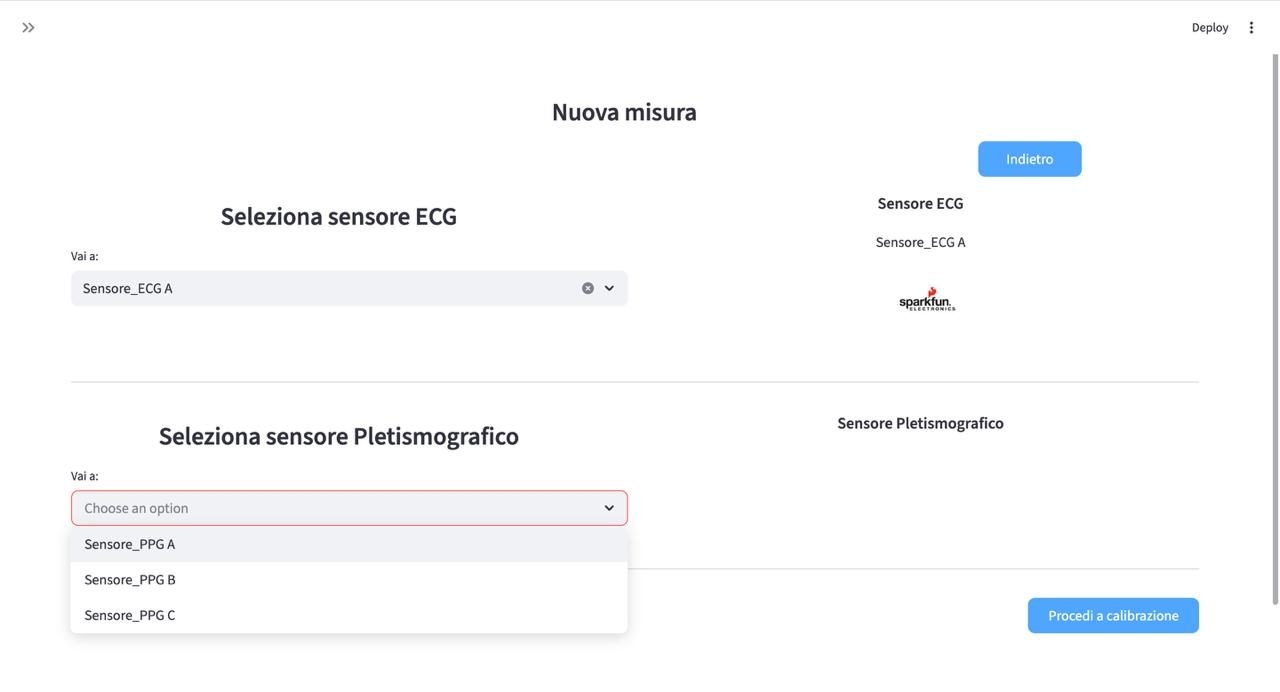
\includegraphics[width=1\linewidth]{Images/foto2.jpeg}
    \caption{Schermata selezione sensori da utilizzare}
    \label{fig:foto2}
\end{figure}
\vspace{\baselineskip}


In Figure~\ref{fig:foto3} è mostrata la schermata successiva. Nella metà sinistra dello schermo viene data all'utente la possibilità di selezionare una calibrazione già salvata  selezionando l'opzione "Calibrazione registrata" oppure crearne una nuova selezionando la voce "Nuova calibrazione". Questo permette di avviare la fase di calibrazione, i cui coefficienti verranno registrati e resi disponibili per le prossime misure. 


Una nota importante: la calibrazione dei dispositivi cuffless per la stima della pressione sanguigna è una procedura complessa, che deve essere svolta in presenza di personale esperto, secondo lo stato dell'arte attuale. In un contesto di applicazione reale, una calibrazione errata potrebbe avere effetti dannosi, portando ad allarmismi o ad ignorare valori preoccupanti.
Per cui, nel contesto di questo progetto, sarebbe poco significativo concedere l'effettiva possibilità da parte dell'utente di compiere una nuova calibrazione.   
Quindi, tale opzione non è stata programmata, ma è comunque mostrata come selezionabile all'interno dell'interfaccia grafica, e potrebbe essere concettualmente realizzabile.   


Nel caso in cui si decida di sfruttare una calibrazione già registrata, la porzione destra dello schermo permette di selezionare tra quelle disponibili, i cui nomi sono assegnati dall'utente stesso in fase di creazione. Una volta selezionata la calibrazione è possibile proseguire alla pagina successiva.
\begin{figure}
    \centering
    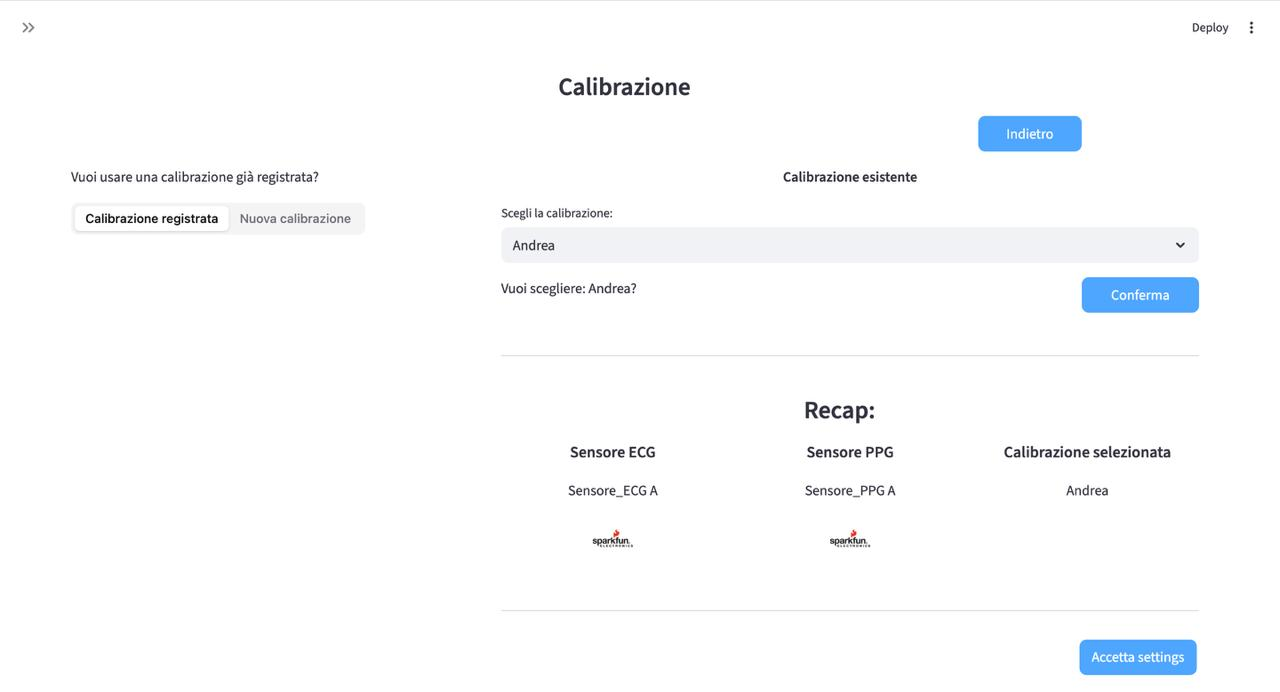
\includegraphics[width=1\linewidth]{Images/foto3.jpeg}
    \caption{Schermata di selezione della calibrazione che si desidera usare per la misura}
    \label{fig:foto3}
\end{figure}
\vspace{\baselineskip}


La pagina in Figura~\ref{fig:foto4} è dedicata alla ricerca e alla connessione dei dispositivi.
Nell'area centrale vengono mostrati i dispositivi (ECG e/o PPG) selezionati, ciascuno rappresentato da un riquadro grafico che include il nome del dispositivo e un’icona Bluetooth. Il colore e l’icona del riquadro variano dinamicamente in base allo stato del dispositivo, permettendo all’utente di comprendere se il sensore è stato individuato o meno.
\begin{figure}
    \centering
    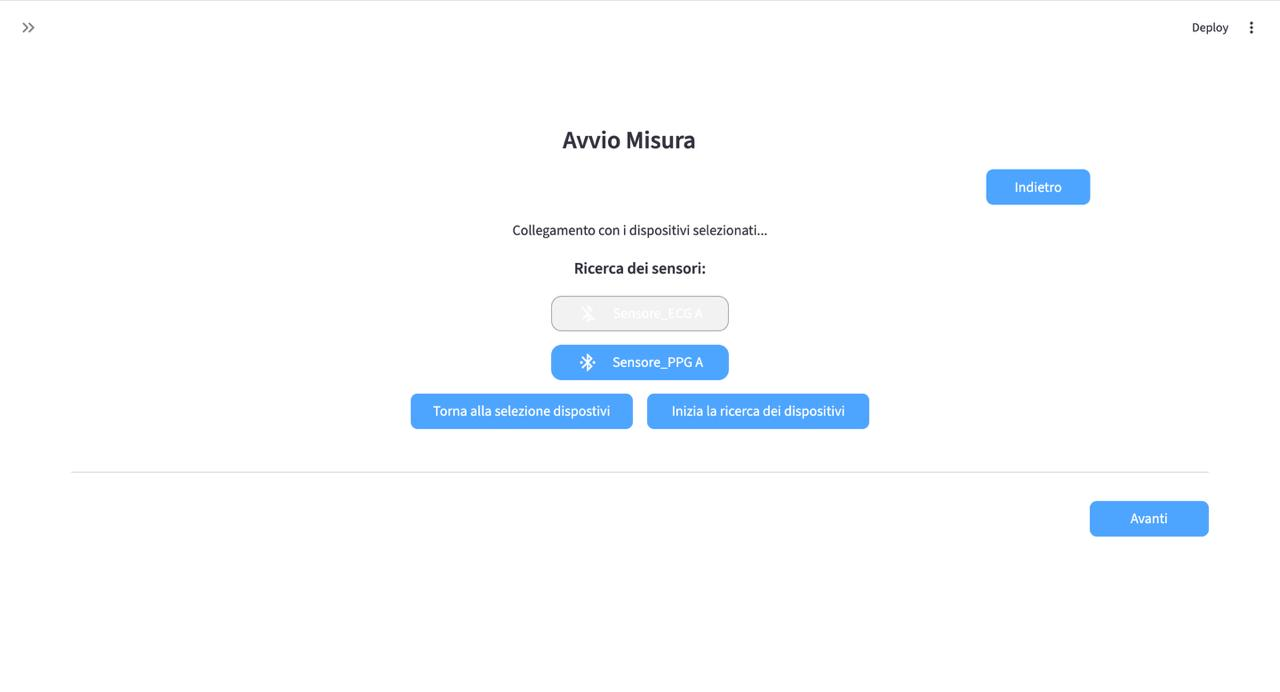
\includegraphics[width=1\linewidth]{Images/foto4.jpeg}
    \caption{Schermata per la connessione tramite BLE dei sensori utilizzati}
    \label{fig:foto4}
\end{figure}
L’utente può avviare la ricerca dei dispositivi tramite il pulsante “Inizia la ricerca dei dispositivi”. Una volta selezionato questo pulsante, l’applicazione esegue una scansione Bluetooth Low Energy (BLE) per individuare i sensori nelle vicinanze. I dispositivi rilevati vengono confrontati con quelli selezionati in precedenza e, in caso di corrispondenza, lo stato dei sensori viene aggiornato automaticamente. Durante questa fase, la pagina fornisce feedback testuale dinamico sullo stato della procedura, informando l’utente sull’avanzamento della ricerca, sull’eventuale individuazione dei sensori, sul tentativo di connessione e sull’esito finale dell’operazione. Qualora un sensore venga individuato ma non risulti ancora connesso, la pagina mette a disposizione un pulsante dedicato che consente all’utente di avviare manualmente il tentativo di connessione.
Nella parte inferiore della pagina è presente una funzione di supporto e debug che consente di effettuare una scansione manuale dei dispositivi Bluetooth disponibili nelle vicinanze utile in caso siano riscontrati problemi nella connessione automatica dei dispositivi.


Una volta collegati i dispositivi desiderati, è possibile procedere all'avvio della misura tramite apposito pulsante, che risulta disabilitato previa connessione di tutti i sensori necessari.
Inoltre, nella parte superiore dell’interfaccia è presente un pulsante di navigazione “Indietro”, che consente di tornare alla fase di calibrazione e di ripristinare lo stato iniziale della ricerca.
Una volta completati questi passaggi, la misura comincia e si passa alla pagina mostrata in Figure~\ref{fig:foto5}, chiamata "Svolgimento Misura". Essa è dedicata alla visualizzazione in tempo reale dei segnali fisiologici acquisiti durante una sessione di misurazione, consentendo all’utente di monitorare l’andamento dei parametri biometrici mentre la misura è in corso. L’intera pagina viene aggiornata automaticamente a intervalli regolari, garantendo una visualizzazione costantemente aggiornata dei dati acquisiti.
\begin{figure}
    \centering
    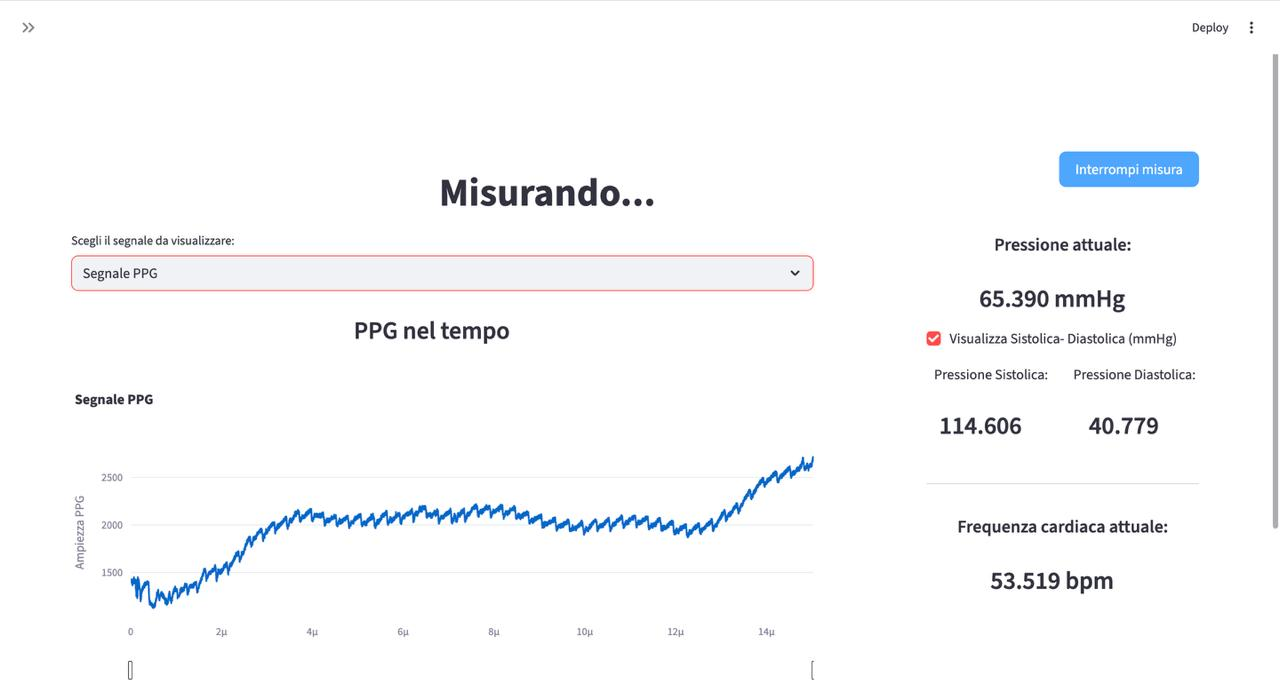
\includegraphics[width=1\linewidth]{Images/foto5.jpeg}
    \caption{Schermata di esecuzione misura. Nell'esempio riportato viene mostrato il grafico del segnale pletismografico.}
    \label{fig:foto5}
\end{figure}
La struttura della pagina è suddivisa in due colonne: la colonna principale è dedicata alla visualizzazione grafica dei segnali, mentre quella laterale fornisce un riepilogo dei valori correnti di pressione e frequenza cardiaca. Nella sezione principale, l’utente può selezionare tramite un menu a tendina quale segnale visualizzare, scegliendo tra ECG, PPG, pressione, frequenza cardiaca, oppure può scegliere di visualizzare simultaneamente tutti i segnali disponibili.
I segnali vengono rappresentati mediante grafici temporali interattivi, che mostrano l’andamento dei valori in funzione del tempo. Per garantire una lettura chiara e focalizzata sui dati più rilevanti, ciascun segnale è visualizzato all’interno di una finestra temporale mobile: per ECG e PPG vengono mostrati gli ultimi secondi di acquisizione, mentre per pressione e frequenza cardiaca viene considerato un intervallo temporale più ampio. In assenza di dati, l’interfaccia informa l’utente che la misura è ancora in fase di avvio.
La colonna laterale della pagina mostra i valori attuali di pressione e frequenza cardiaca, calcolati come media dei dati più recenti disponibili. Questi valori vengono aggiornati automaticamente e consentono all’utente di avere un’indicazione immediata e sintetica dello stato corrente durante la misurazione.
Nella parte superiore è inoltre presente il pulsante “Interrompi misura”, che permette all’utente di terminare l’acquisizione e passare alla fase di conclusione della misura prima che i dati di questa vengano salvati.

La pagina "Fine Misura", mostrata in Figure~\ref{fig:foto6}, rappresenta la fase conclusiva del processo di acquisizione dei segnali e ha lo scopo di consentire all’utente di analizzare i risultati della misurazione e procedere al salvataggio dei dati. In questa sezione, i segnali acquisiti durante la sessione vengono resi disponibili in forma grafica e possono essere esaminati in modo dettagliato prima della loro memorizzazione definitiva.
La struttura della pagina è organizzata in tre colonne principali. La colonna sinistra è dedicata alla selezione dei segnali da visualizzare e presenta un insieme di checkbox che permettono all’utente di scegliere uno o più segnali tra ECG, PPG, pressione e frequenza cardiaca. Questa selezione influenza dinamicamente il contenuto della sezione centrale della pagina.
Nella colonna centrale vengono mostrati i grafici temporali relativi ai segnali selezionati. Ogni segnale è rappresentato mediante un grafico interattivo che consente lo scorrimento lungo l’asse temporale, permettendo un’analisi dettagliata dell’andamento del segnale nel corso della misurazione. La possibilità di visualizzare più segnali contemporaneamente consente un confronto diretto tra le diverse grandezze fisiologiche acquisite.
La colonna destra è dedicata all’inserimento delle informazioni di contesto associate alla misura. In questa sezione l’utente può selezionare la data in cui è stata effettuata la misurazione tramite un calendario interattivo e indicare il periodo della giornata in cui essa ha avuto luogo (mattino, pomeriggio o sera). Queste informazioni vengono utilizzate per contestualizzare correttamente la misura e facilitarne la successiva consultazione nello storico.
Nella parte superiore dell’interfaccia è presente il pulsante “Salva”, la cui attivazione è subordinata alla corretta compilazione delle informazioni richieste. In particolare, il pulsante rimane disabilitato finché l’utente non seleziona una data dal calendario e non indica il periodo della giornata in cui è stata effettuata la misura.
\begin{figure}
    \centering
    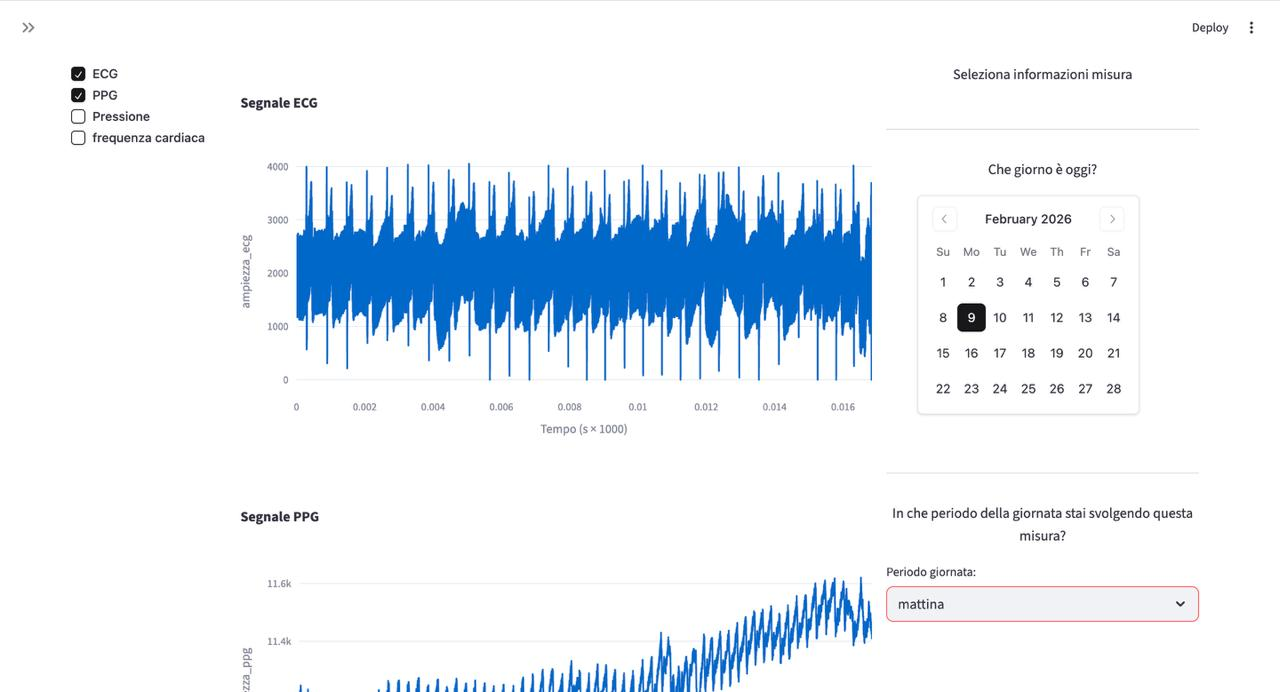
\includegraphics[width=1\linewidth]{Images/foto6.jpeg}
    \caption{Schermata fine misura per visualizzare la misura effettuata sui vari segnali acquisiti e specificare il giorno e periodo in cui è stata effettuata.}
    \label{fig:foto6}
\end{figure}


\subsection{Consultazione storico dati paziente}
La pagina "Storico Misure", mostrata nelle figure~\ref{fig:foto7} e \ref{fig:foto8}, fornisce all’utente un’interfaccia per consultare le misure precedentemente registrate. La visualizzazione è focalizzata sulla misura singola, con la possibilità di analizzare i segnali raccolti, tra cui pressione arteriosa, frequenza cardiaca, ECG e PPG, tramite selezione checkbox per ciascun segnale.

La colonna principale permette di selezionare una misura specifica da un menu a tendina, nel quale ogni voce indica l’identificativo della misura e la data e ora di acquisizione. Una volta selezionata, l’utente può visualizzare i segnali disponibili come grafici interattivi, mentre informazioni contestuali come il periodo della giornata della misura e il nome della calibrazione associata vengono mostrate in modo chiaro.

Attraverso la checkbox “Visualizza statistiche”, l’utente può abilitare la visualizzazione di dati aggregati relativi alle misure registrate. In questa modalità, la pagina mostra statistiche globali quali numero di sessioni registrate, pressione e frequenza cardiaca media, minima e massima nell'intervallo temporale selezionato. Ulteriori dettagli sulla pressione sistolica e diastolica possono essere attivati opzionalmente per fornire un’analisi più approfondita.

Le statistiche possono essere filtrate in base a due criteri: l’intervallo temporale di interesse e il periodo della giornata in cui le misure sono state effettuate. Questo permette di analizzare l’andamento della pressione e della frequenza cardiaca sia complessivamente nell’intervallo selezionato, sia specificamente per mattina, pomeriggio o sera, fornendo un quadro chiaro e flessibile dell’evoluzione dei dati del paziente.
\begin{figure}
    \centering
    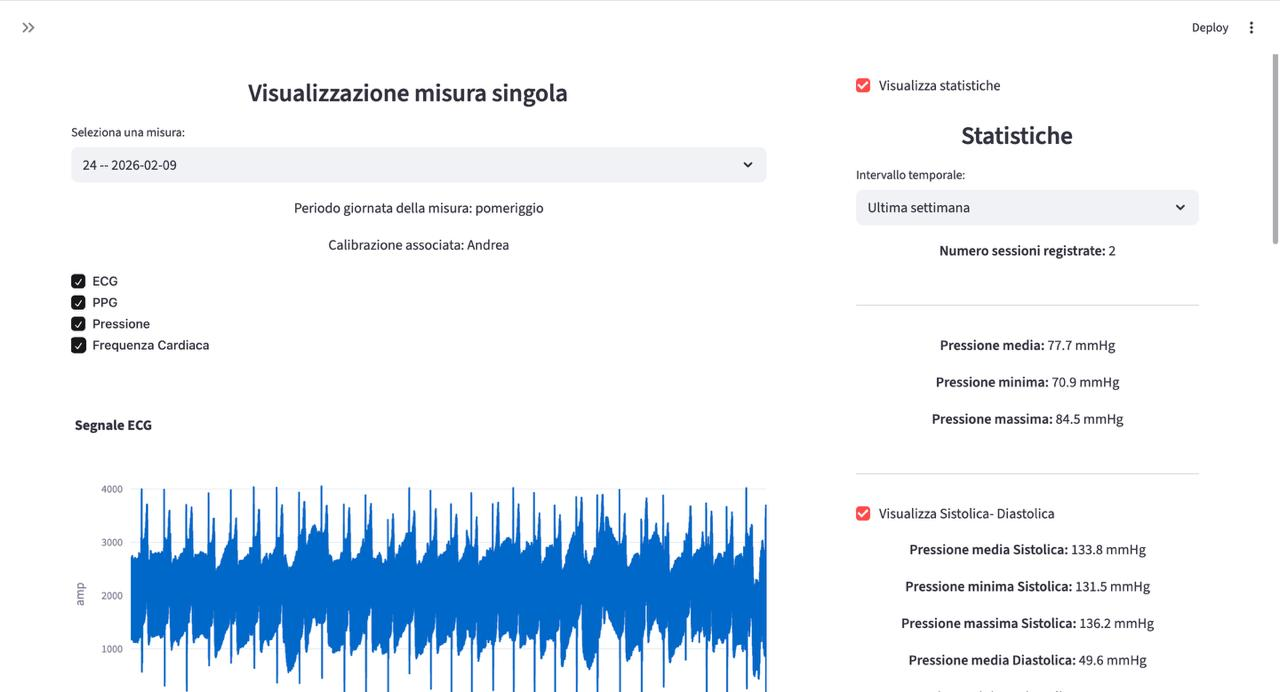
\includegraphics[width=1\linewidth]{Images/foto7.jpeg}
    \caption{Parte superiore della schermata storico delle misure}
    \label{fig:foto7}
\end{figure}
\begin{figure}
    \centering
    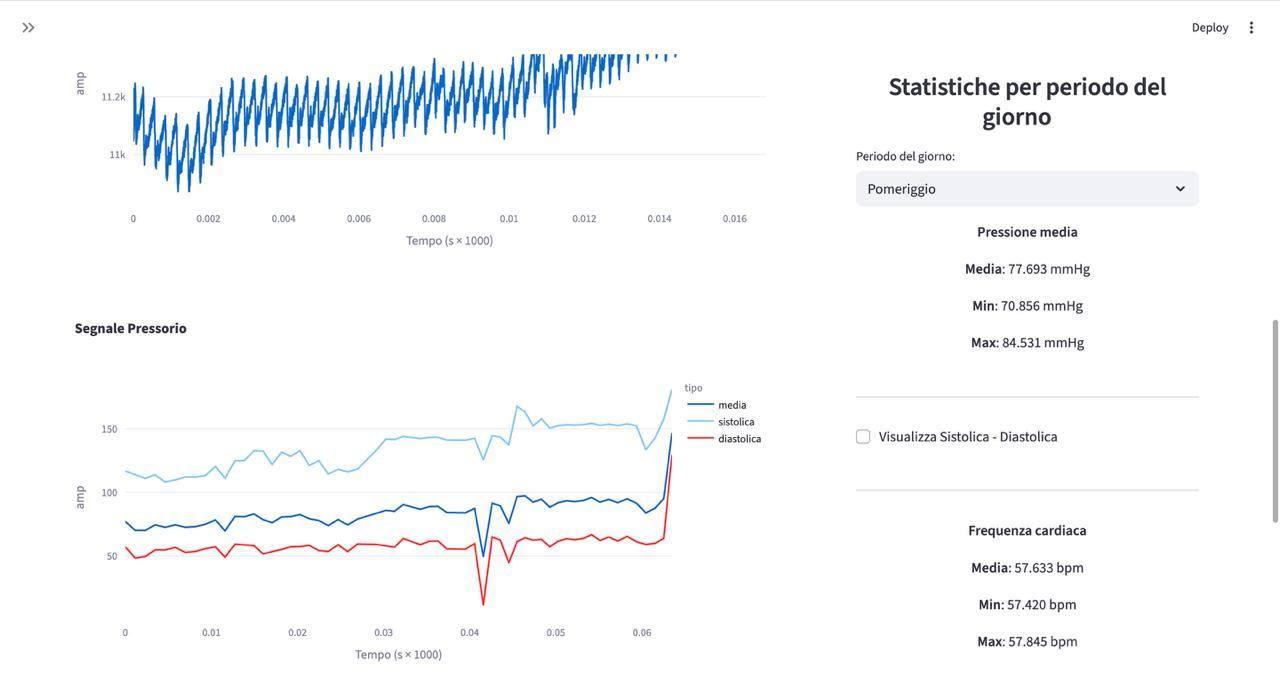
\includegraphics[width=1\linewidth]{Images/foto8.jpeg}
    \caption{Parte inferiore della schermata storico delle misure}
    \label{fig:foto8}
\end{figure}



\subsection{Modifica dati profilo utente}
La pagina Profilo Utente, mostrata in Figure~\ref{fig:foto10}, consente all’utente di visualizzare, modificare e gestire tutte le informazioni personali associate al proprio account. Essa fornisce un’interfaccia chiara e organizzata in due sezioni principali: la gestione dell’immagine del profilo e la gestione dei dati personali e di contatto.
Nella colonna sinistra viene mostrata l’immagine del profilo. Se l’utente non ha ancora caricato una propria immagine, viene visualizzata un'immagine di default. È possibile caricare una nuova immagine tramite un uploader integrato, che aggiorna immediatamente l’immagine memorizzata nel database e fornisce un feedback visivo di conferma.
La colonna destra mostra i dati personali dell’utente, inclusi nome, cognome, data di nascita e sesso. I campi peso e altezza sono inizialmente disabilitati, ma possono essere modificati entrando in modalità di editing. In questa modalità l’utente può aggiornare i valori, confermarli tramite il pulsante "Salva dati" o annullare le modifiche. Il sistema effettua controlli di validità sui valori inseriti, assicurando che peso e altezza siano maggiori di zero.
A questa segue la sezione dedicata ai numeri di contatto, comprendente il numero di telefono e un contatto ICE (in caso di emergenza). Anche questi campi possono essere modificati in modalità editing, con validazione dei dati inseriti affinché contengano solo cifre.
Infine, la pagina include una sezione per il cambio della password, accessibile tramite un expander. L’utente deve inserire la password attuale, la nuova password e confermarla. Vengono effettuati controlli di coerenza e di sicurezza, come la corrispondenza delle nuove password e una lunghezza minima di sei caratteri, e viene fornito un feedback immediato sull’esito dell’operazione.
\begin{figure}
    \centering
    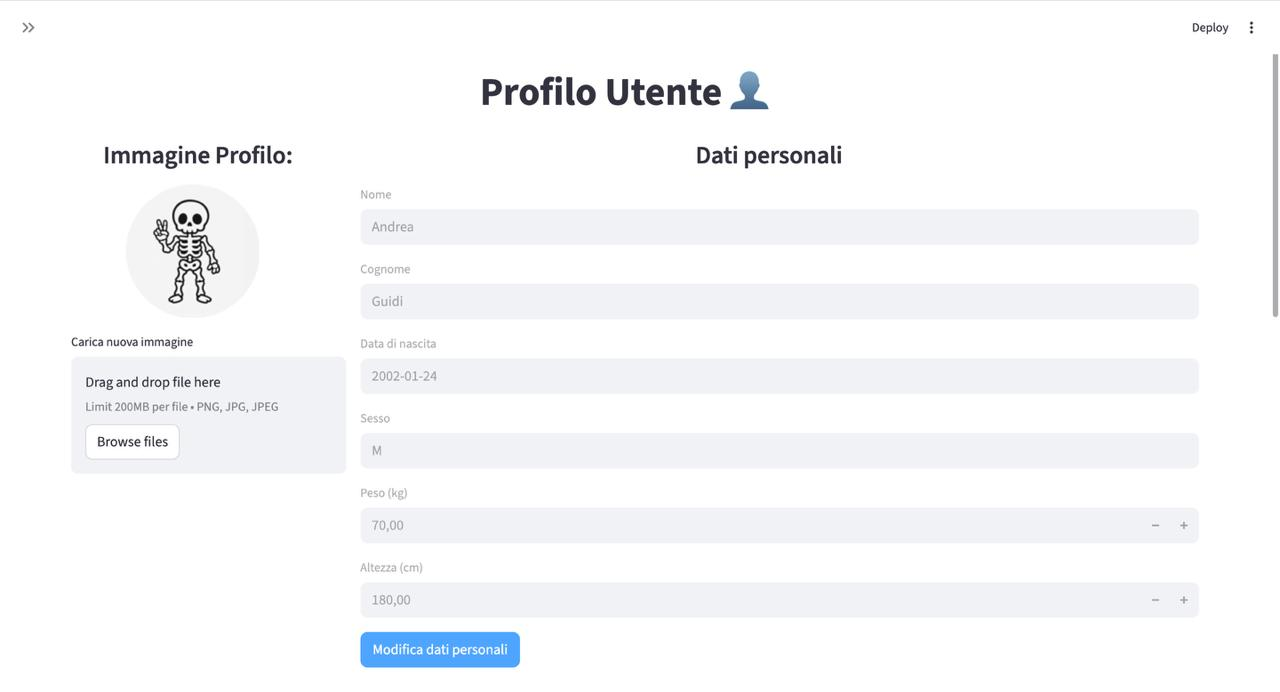
\includegraphics[width=1\linewidth]{Images/foto10.jpeg}
    \caption{Schermata pagina profilo utente con possibilità di modifica dati personali.}
    \label{fig:foto10}
\end{figure}

\subsection{Contatto supporto tecnico}
\label{sssec:Contatto supporto tecnico}
La pagina "Informazioni", mostrata in Figure~\ref{fig:foto11}, fornisce una panoramica generale sull’applicazione e sulle sue funzionalità principali, fungendo da guida introduttiva per l’utente. Essa espone in maniera chiara e sintetica gli scopi dell’applicazione, in particolare il monitoraggio sicuro della pressione arteriosa.
La pagina è costituita da un testo centrato che descrive le funzionalità principali dell’applicazione. Tra queste si evidenziano la possibilità di registrarsi e effettuare login sicuri, aggiornare il proprio profilo, caricare un’immagine personale, modificare i numeri di contatto e cambiare la password. La pagina dedica inoltre una sezione alla sicurezza dei dati, informando l’utente che tutte le informazioni sono memorizzate in modo sicuro e che le password sono criptate, garantendo la privacy. Inoltre è presente un riferimento al supporto tecnico che l'utente è libero di contattare per eventuali necessità o chiarimenti.
\begin{figure}
    \centering
    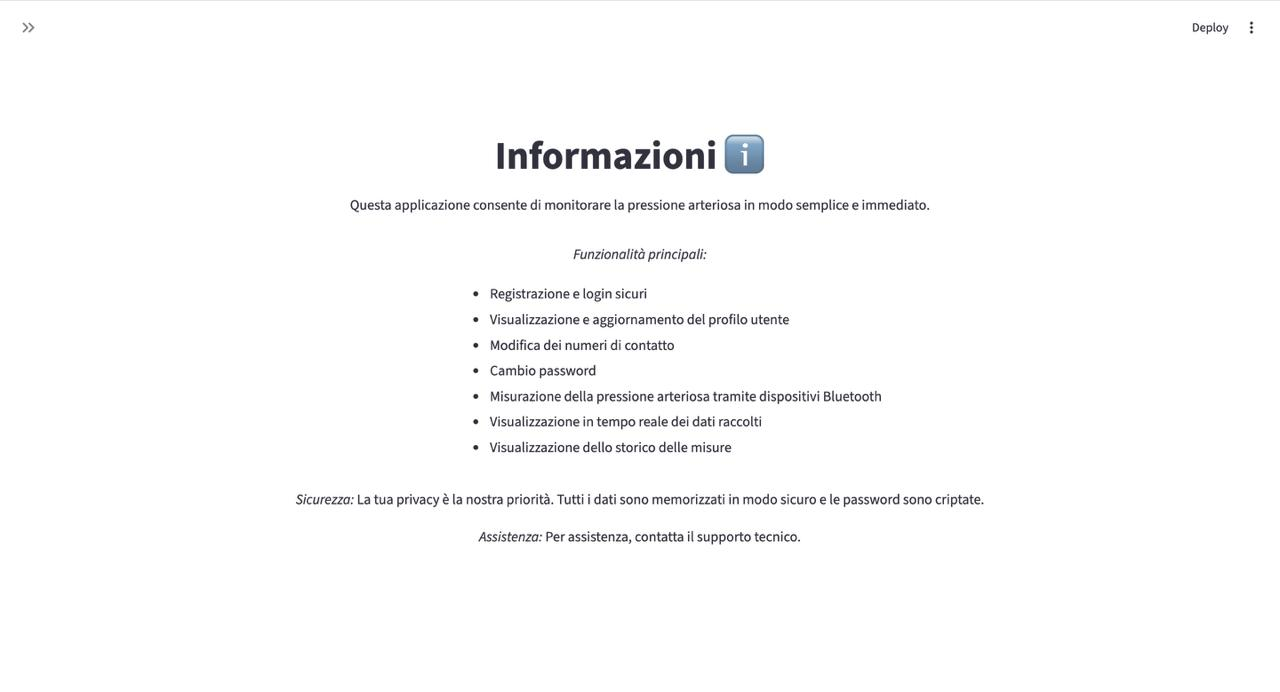
\includegraphics[width=1\linewidth]{Images/foto11.jpeg}
    \caption{Schermata contatti per richiedere supporto tecnico}
    \label{fig:foto11}
\end{figure}

\subsection{Consulto domande frequenti}
La pagina "FAQ", mostrata in Figure~\ref{fig:foto9}, ha lo scopo di fornire informazioni di base all’utente riguardo al monitoraggio della pressione arteriosa e alle condizioni di salute correlate, come l’ipertensione. Essa rappresenta una sezione informativa e non interattiva, utile per educare l’utente e rispondere a dubbi comuni, migliorando la consapevolezza riguardo alla salute cardiovascolare e a incentivare comportamenti preventivi. Le domande sono indicate con la sigla D: e le risposte con R:, garantendo una distinzione immediata tra quesito e spiegazione. Alcune risposte contengono link esterni, che permettono all’utente di approfondire ulteriormente le informazioni direttamente dalle fonti ufficiali, come l’Organizzazione Mondiale della Sanità.
\begin{figure}
    \centering
    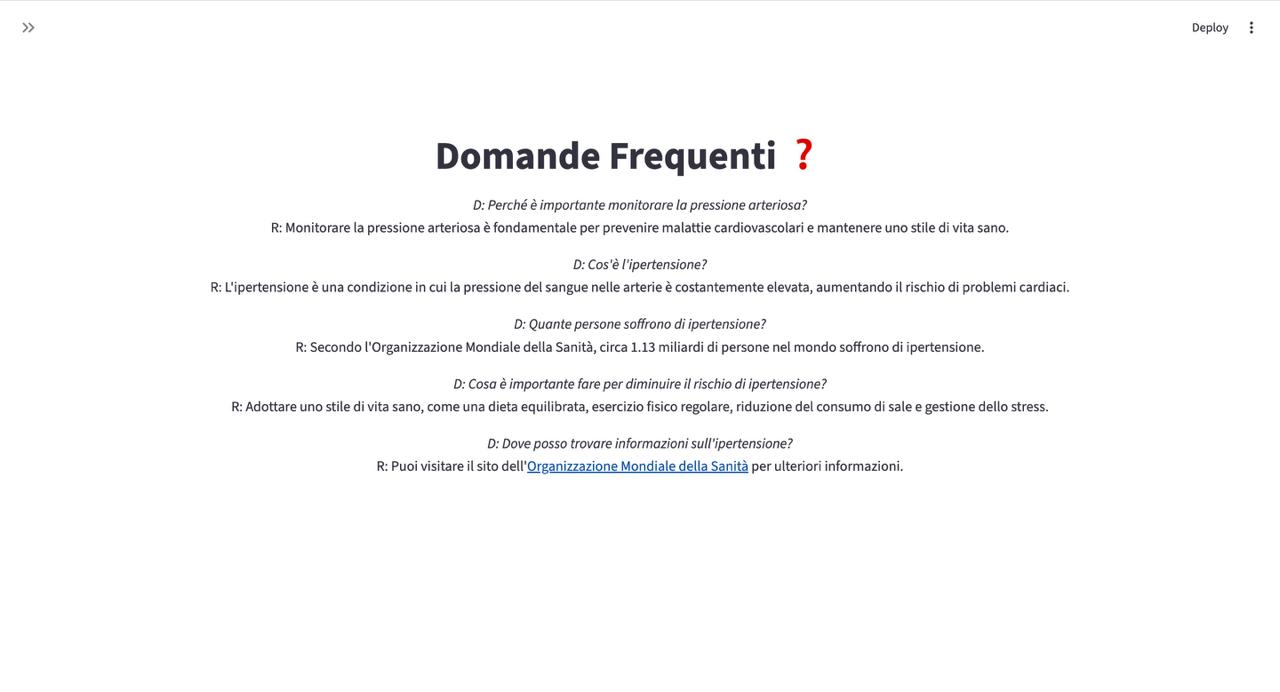
\includegraphics[width=1\linewidth]{Images/foto9.jpeg}
    \caption{Schermata domande frequenti con link a sito ufficiale OMS.}
    \label{fig:foto9}
\end{figure}

\subsection{Logout}
Al fine di garantire la sicurezza e confidenzialità dei dati sensibili è sempre necessaria la funzione di logout per garantire l'impossibilità di accedere ai dati personali del paziente anche in caso di accesso ai device sui quali l'applicazione sia consultata.

\section{Case}
\label{Sezione Case}
Un chiaro obiettivo di questo progetto era quello di sviluppare un dispositivo \textit{wearable}, quindi di rendere indossabili i diversi moduli necessari, tenendo conto dei punti di applicazione dei sensori e cercando di minimizzare la lunghezza dei fili. Le prospettive future prevederebbero la stampa della PCB e quindi un miglioramento dell'ergonomicità del dispositivo, ma il primo prototipo di case è stato sviluppato basandosi sul circuito su millefori.  
\subsection{Case modulo ECG e microcontrollore}


% --- Primo blocco ---
\begin{figure}[H]
    \begin{minipage}{0.4\textwidth}
        \centering
        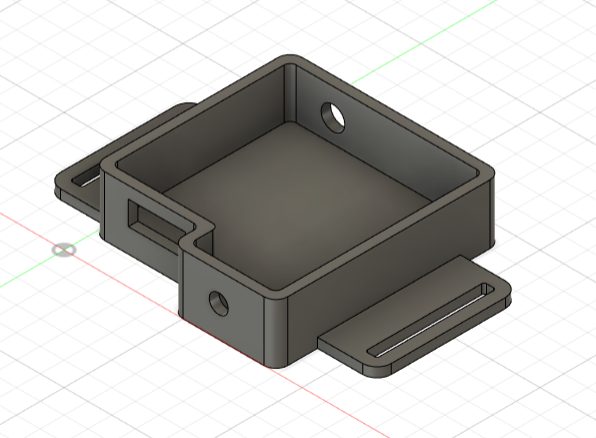
\includegraphics[width=\textwidth]{CaseECGzxy.png}
        \caption{Case ECG}
        \label{fig:case_ecg_1}
    \end{minipage}
    \hfill
    \begin{minipage}{0.55\textwidth}
        Le alette laterali fungono da passanti per permettere al case (in figura \ref{fig:case_ecg_1}) di essere indossato tramite una comune cintura. Questo permette di agganciare fermamente il case all'altezza della vita, in maniera tale che gli elettrodi possano facilmente raggiungere i punti di applicazione sul petto e il peso e l'ingombro del dispositivo non siano d'impedimento. Il lato dalla parte della scheda breakout deve guardare verso il basso quando il case viene indossato alla cintura. Esso presenta uno scalino che permette al connettore per l'alimentazione del microcontrollore di fuoriuscire parzialmente per connettere il dispositivo e ricaricare la batteria via cavo. Lo scalino presenta anche un foro per connettere e consentire aggiustamenti della batteria. Il lato che guarda in alto invece presenta un foro circolare per inserire comodamente il jack degli elettrodi ECG. La figura \ref{fig:ECGreal} mostra la disposizione degli elementi all'interno del case e l'alloggiamento della batteria. 
    \end{minipage}
\end{figure}



% --- Secondo blocco ---
\begin{figure}[H]
    \begin{minipage}{0.4\textwidth}
        \centering
        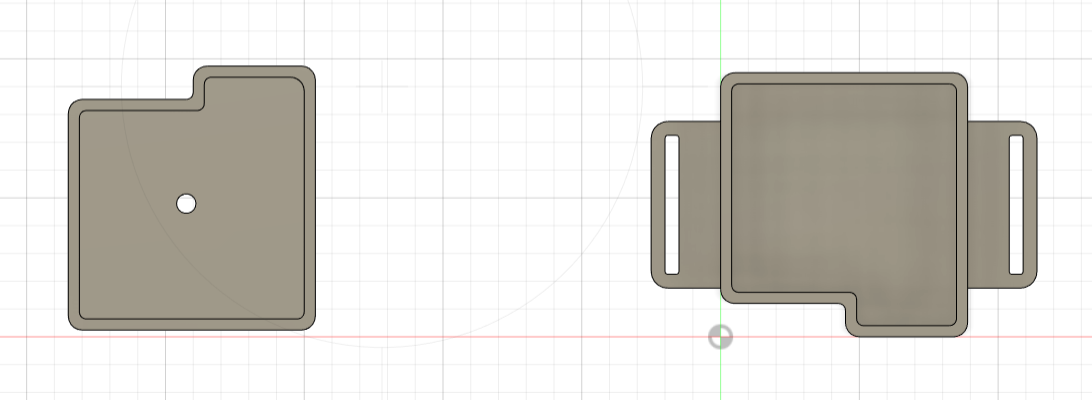
\includegraphics[width=\textwidth]{CaseECGvistadallalto.png}
        \caption{Case ECG vista dall'alto}
        \label{fig:case_ecg_alto}
    \end{minipage}
    \hfill
    \begin{minipage}{0.55\textwidth}
        La vista dall'alto (in figura \ref{fig:case_ecg_alto}) include anche il coperchio ad incastro, che presenta un foro in corrispondenza del led rosso collegato al pin del modulo ECG. Tale led segnala eventuali problemi di connessione (è collegato al pin di \textit{Leads-off detect}): nel caso di disconnessione, la luce del led rosso è chiaramente visibile anche dall'esterno. 
    \end{minipage}
\end{figure}

\begin{figure}[H]
    \centering
    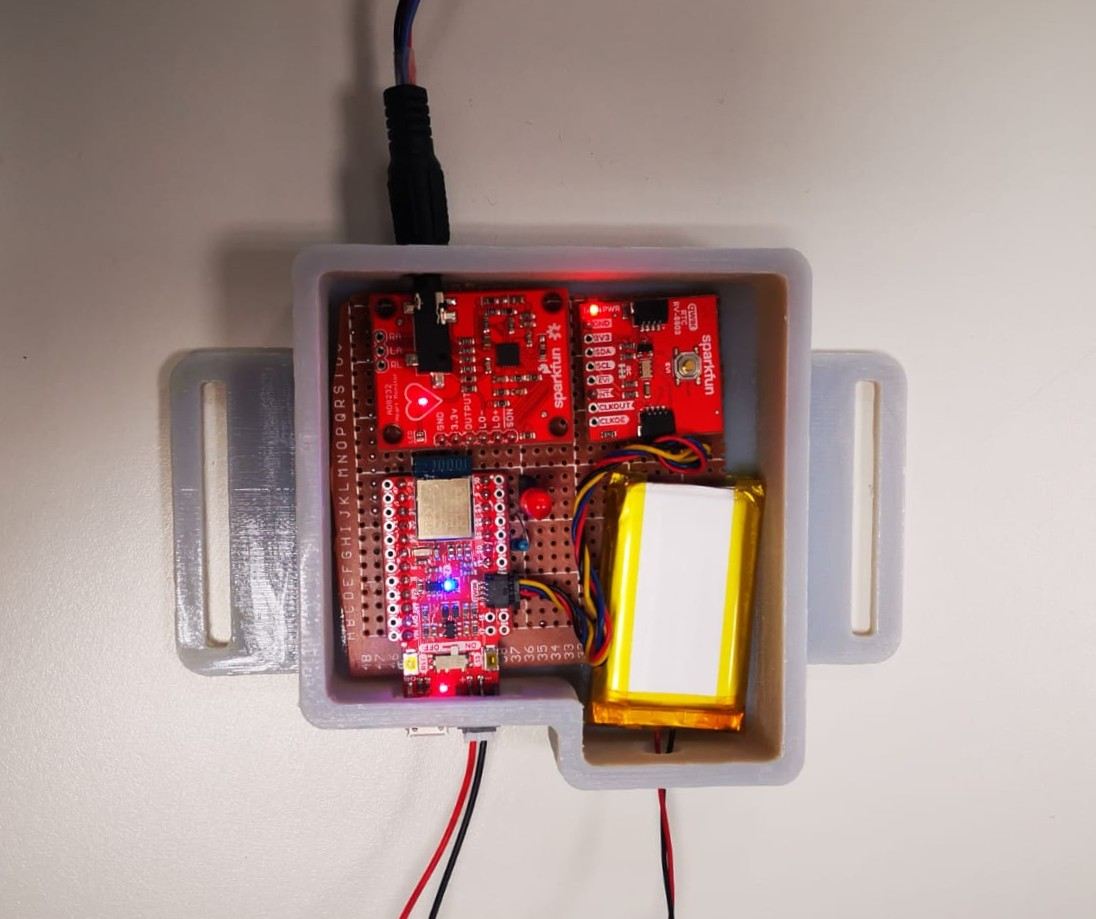
\includegraphics[width=0.4\textwidth]{ECGreal.jpeg}
    \caption{Case per il modulo ECG}
    \label{fig:ECGreal}
\end{figure}


\subsection{Case modulo PPG}
\begin{figure}[H]
    \begin{minipage}{0.4\textwidth}
        \centering
        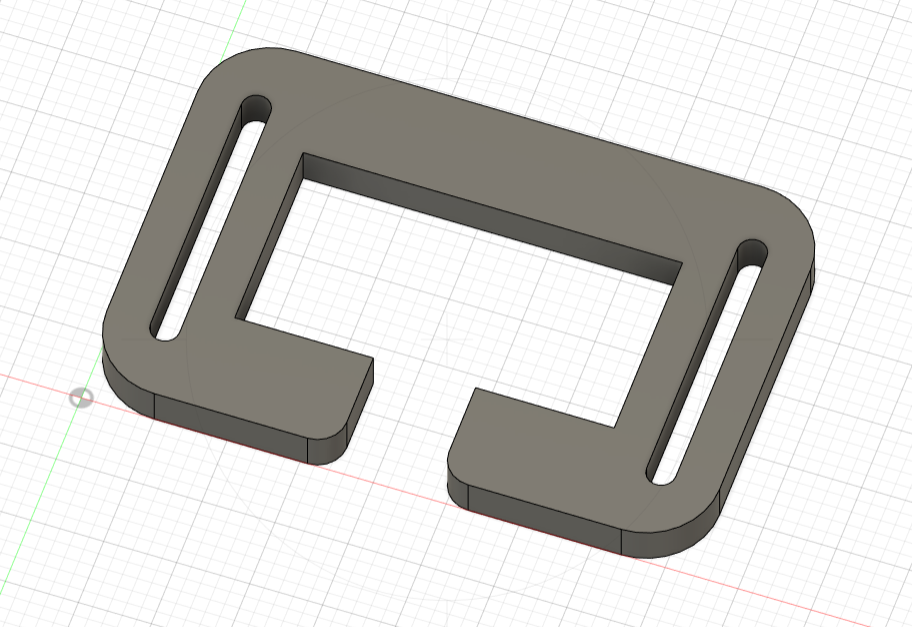
\includegraphics[width=\textwidth]{CasePPG.png}
        \caption{Case PPG}
        \label{fig:case_ppg}
    \end{minipage}
    \hfill
    \begin{minipage}{0.55\textwidth}
        Il case per il modulo PPG (in figura \ref{fig:case_ppg}) consiste in una placchetta che permette di incastrare il modulo al suo interno (come mostrato in figura \ref{fig:PPGreal}), e fissare il dispositivo con il sensore a contatto con la pelle. Le due fessure laterali consentono il passaggio di una fascetta elastica per il fissaggio del dispositivo al piede.
    \end{minipage}
\end{figure}
\begin{figure}[H]
    \centering
    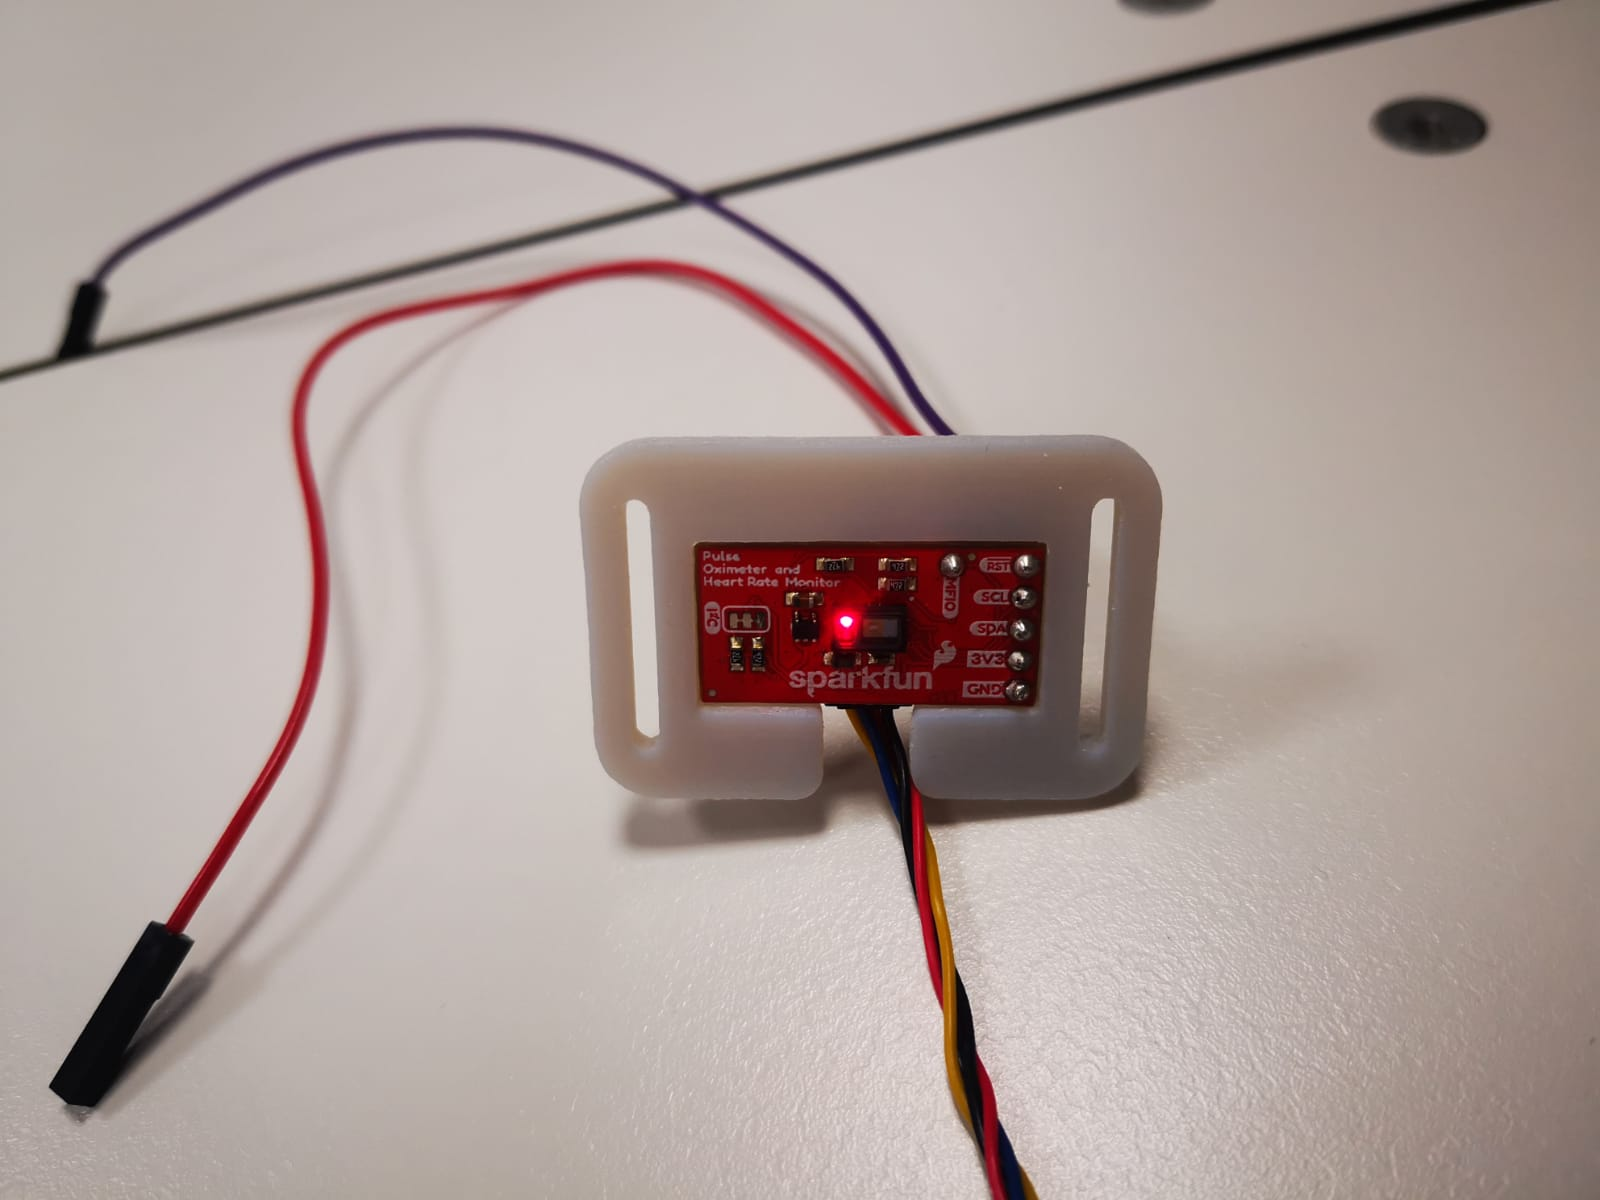
\includegraphics[width=0.4\textwidth]{PPGreal.jpeg}
    \caption{Case per il sensore PPG}
    \label{fig:PPGreal}
\end{figure}


\subsection{Case modulo RTC e microcontrollore}
\begin{figure}[H]
    \begin{minipage}{0.4\textwidth}
        \centering
        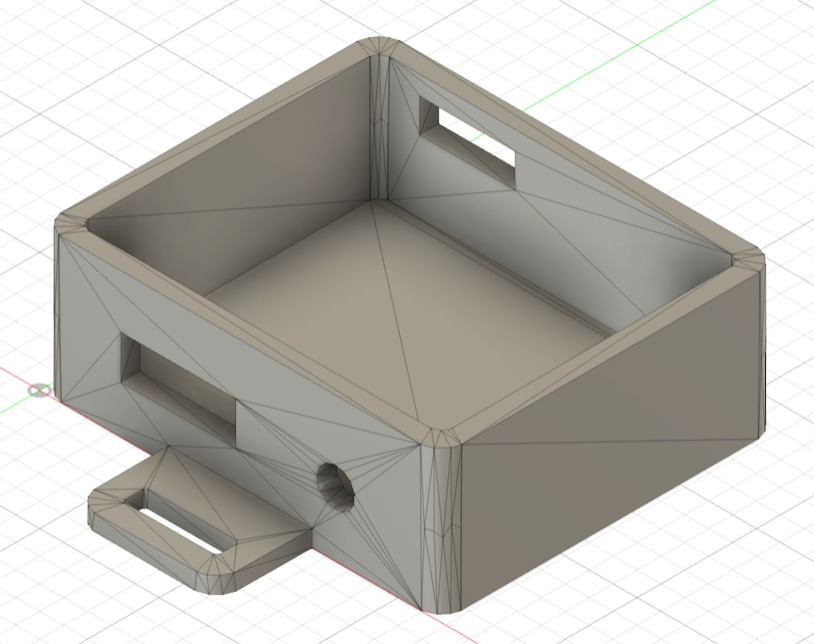
\includegraphics[width=\textwidth]{PPGxyz.jpeg}
        \caption{Case RTC e microcontrollore per PPG}
        \label{fig:case_rtc_xyz}
    \end{minipage}
    \hfill
    \begin{minipage}{0.55\textwidth}
        Il case contenente il modulo RTC e il microcontrollore per l'acquisizione della PPG (in figura \ref{fig:case_rtc_xyz}), come quello per l'ECG, consiste  in un dispositivo chiudibile tramite coperchio: ha però delle dimensioni minori per poter essere indossato alla caviglia. Esattamente come il case per il modulo ECG, esso presenta delle cavità sulle pareti che permettono di connettere la batteria e il modulo RTC, come visibile dalla figura \ref{fig:RTCreal}.
    \end{minipage}
\end{figure}
\begin{figure}[H]
    \centering
    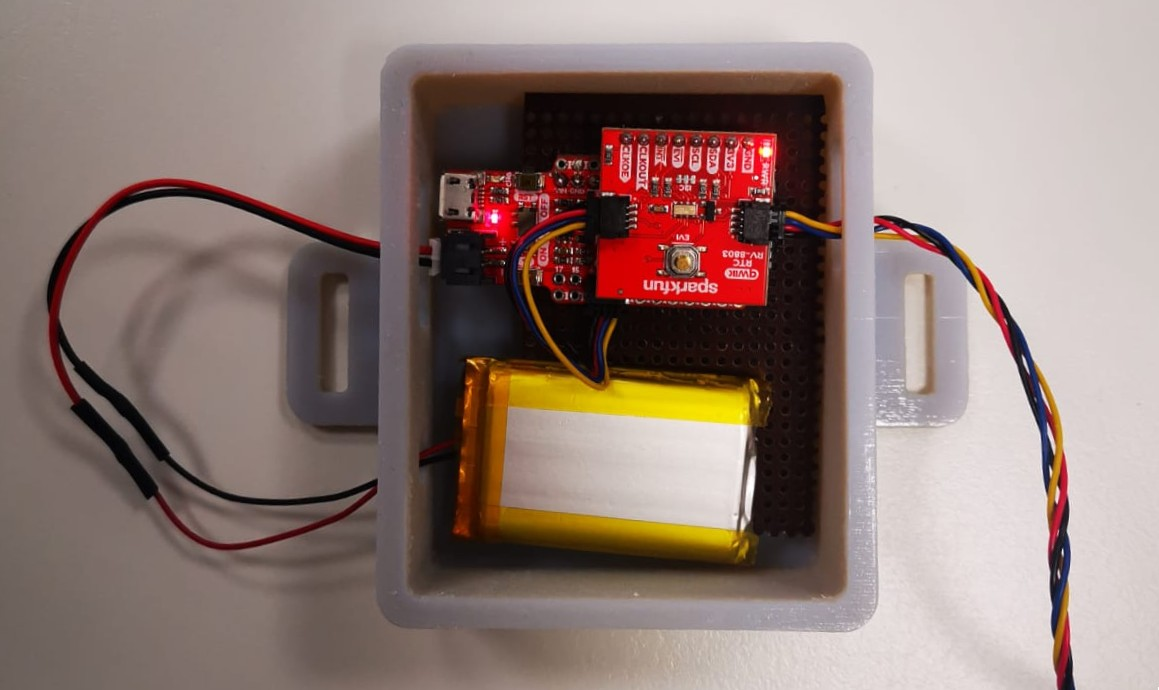
\includegraphics[width=0.4\textwidth]{RTCreal.jpeg}
    \caption{Case per il modulo RTC e microcontrollore del sensore PPG}
    \label{fig:RTCreal}
\end{figure}

Ciascun case è provvisto di una fascia elastica con delle fibbie in plastica che ne permettono la regolazione per essere indossato da chiunque. 


\section{Calibrazione}
\label{Sezione Calibrazione}
La calibrazione del dispositivo è implementata attraverso un software dedicato in Python con l'obiettivo di trasformare i parametri bioelettrici grezzi in stime della pressione arteriosa. 

In letteratura, il PAT viene utilizzato nei dispositivi \textit{wearable} per stimare la pressione sistolica (SYS), diastolica (DIA) e media (MAP,  $MAP = DIA + \frac{1}{3}(SYS - DIA)$). Sebbene si sia evidenziato soprattutto il legame tra il PAT e la pressione sistolica \cite{Panula2023}, anche le relazioni tra questa quantità e la pressione diastolica \cite{Finnegan2021} e media \cite{Pilz2022-lq} sono state esplorate, dunque nell'ambito di questo progetto è stato deciso di calibrare tutte e tre le pressioni.


Per mappare correttamente il comportamento del sensore, sono stati indotti cambiamenti pressori significativi attraverso stimoli diversificati \cite{Panula2023} sul soggetto: l'assunzione di caffeina \cite{Nurminen1999-vg}, l'esecuzione di attività fisica, il consumo di pasti e variazioni posturali \cite{Xie_Effects}. 
Il software gestisce interattivamente la procedura di acquisizione dei punti di calibrazione: per ogni condizione fisiologica indotta, l'utente avvia manualmente una registrazione (di circa 60 secondi) dei segnali provenienti dalle boards tramite BLE. Durante questa fase deve essere anche registrata la pressione attraverso lo sfigmomanometro di riferimento che viene successivamente inserita a terminale. 


Infine, lo script elabora i dati ricevuti e applica dei limiti di accettabilità fisiologica (derivanti da letteratura e prove sperimentali nel nostro set-up) per garantire la pulizia del segnale: il PAT viene considerato valido solo se compreso tra 300 ms e 800 ms, mentre l'intervallo tra i battiti (intervallo RR) deve rientrare nel range tra 0.3 s (200 BPM) e 1.5 s (40 BPM): tali filtri sono essenziali per eliminare eventuali artefatti da movimento o falsi rilevamenti che comprometterebbero la precisione del modello finale.


Il software infatti calcola la mediana dei PAT e la media dei BPM registrati in quel segmento e salva il punto di calibrazione (composto da PAT, BPM e BP manuale) in una lista. Una volta raccolto un numero sufficiente di punti in diverse condizioni, lo script utilizza il metodo dei minimi quadrati per determinare i coefficienti personalizzati delle varie relazioni testate. Questi coefficienti verranno poi utilizzati per generare la pressione arteriosa istantanea per ogni battito.


Inizialmente, l'approccio si è basato su modelli a singola variabile, testando una relazione lineare tra Pulse Arrival Time (PAT) e pressione (BP) \cite{lazazzera2019}:
\begin{equation}
    BP = a \cdot PAT + b
\end{equation}
Tuttavia, i test sperimentali hanno evidenziato che queste approssimazioni non erano sufficienti a catturare la complessità della risposta emodinamica. Dall'analisi dei dati è infatti emerso chiaramente che la frequenza cardiaca non poteva essere trascurata: a parità di PAT, variazioni di BPM influenzano sensibilmente la pressione, rendendo necessario un modello più sofisticato.


Di conseguenza, la logica di calcolo è stata spostata su una regressione lineare multipla basata sull'equazione \cite{lazazzera2019}:
\begin{equation}
    BP = a \cdot PAT + b \cdot BPM + c
\end{equation}
che, per le tre stime diventa:
\begin{equation}
\begin{cases} 
    SYS = a_{sys} \cdot PAT + b_{sys} \cdot BPM + c_{sys} \\
    DIA = a_{dia} \cdot PAT + b_{dia} \cdot BPM + c_{dia} \\
    MAP = a_{map} \cdot PAT + b_{map} \cdot BPM + c_{map}
\end{cases}
\end{equation}
Questo modello permette di pesare correttamente il contributo sia del tempo di arrivo dell'onda che della frequenza cardiaca nel calcolo della pressione Sistolica (SYS), Diastolica (DIA) e Media (MAP)


In genere, 4 punti misurati in un lasso temporale di 30 minuti sono risultati sufficienti per una stima abbastanza accurata.

È stata testata anche una relazione più complessa, che prevede sempre di considerare PAT e BPM \cite{Zhou2023}: \begin{equation}
    BP = \frac{a}{PAT^2} + \frac{b}{BPM^2} + c
\end{equation}
Questa però non ha evidenziato particolari miglioramenti, avendo contemporaneamente un costo computazionale più elevato, e di conseguenza è stata scartata.

\section{Risultati: prestazioni real-time}
\subsection{Analisi e Stima dei Ritardi del Sistema}
La stima della pressione basata sul PAT (Pulse Arrival Time) richiede la misura di intervalli di tempo molto piccoli, nell'ordine dei millisecondi. Poiché il nostro sistema utilizza due schede separate che non sono collegate fisicamente tra loro, non condividono lo stesso orologio. È quindi fondamentale capire quali ritardi possono influenzare la sincronizzazione tra le due schede, per distinguere gli errori che possiamo correggere da quelli che potrebbero peggiorare la stima.

\subsubsection{PEP: Errore Fisiologico}
La prima componente temporale analizzata non è di natura strumentale ma fisiologica: il \textit{Pre-Ejection Period (PEP)}. Questo intervallo rappresenta il ritardo elettromeccanico che intercorre tra la depolarizzazione ventricolare (segnalata dal picco R dell'ECG) e l'apertura della valvola aortica, momento in cui l'onda sfigmica viene effettivamente generata ed espulsa nel sistema arterioso.

Poiché il dispositivo sviluppato misura il Pulse Arrival Time (PAT), definito come la somma del tempo di transito dell'impulso (PTT) e del PEP stesso, quest'ultimo costituisce un ritardo intrinseco alla metodologia di misura scelta. Il suo valore non è costante e la sua variabilità dipende dallo stato fisiologico del soggetto, influenzata principalmente dalla contrattilità cardiaca e dal post-carico ventricolare.

Da un punto di vista strettamente fisico, il PEP rappresenterebbe una fonte di errore, in quanto non è correlato direttamente alla velocità di propagazione dell'onda sfigmica lungo i vasi e quindi alla rigidità arteriosa. Tuttavia, come evidenziato nello stato dell'arte, in contesti di monitoraggio reale il PEP agisce sinergicamente con il PTT. È stato dimostrato che l'attivazione del sistema nervoso simpatico, che induce un aumento della pressione arteriosa, provoca contestualmente un aumento della contrattilità cardiaca e quindi una riduzione del PEP. Poiché anche il PTT diminuisce all'aumentare della pressione (a causa dell'irrigidimento vascolare), le variazioni dei due parametri avvengono nella stessa direzione. Questo fenomeno amplifica la variazione complessiva del PAT misurato, migliorando potenzialmente la sensibilità del sistema nel rilevare i cambiamenti pressori rispetto alla sola misura del tempo di transito \cite{Xie_Effects}.

Oltre a ciò, va sottolineato il fatto che una delle scelte progettuali è stata quella di posizionare il sensore PPG sul piede e non per esempio sul polso, proprio per diminuire il rapporto PEP/PAT così da minimizzare il suo effetto sulla misura.


\subsubsection{Ritardo di Avvio Bluetooth}
Un'altra fonte di ritardo avviene nel momento in cui inizia la misurazione. Il computer invia il comando di "Start" alle due schede tramite Bluetooth. Poiché questo invio non è istantaneo e avviene in sequenza, i clock interni (RTC) dei due dispositivi non partono nello stesso identico istante. Questo crea un piccolo sfasamento temporale (offset) tra i due segnali.

Tuttavia, questo è un disallineamento temporale costante (offset) che rimane fisso per tutta la durata della sessione di misura, fintanto che la connessione rimane attiva. Di conseguenza, questo ritardo è compensato dalla procedura di calibrazione. Il modello di regressione utilizzato per la stima della pressione, infatti, assorbe automaticamente questo offset costante all'interno del termine noto dell'equazione, compensando di fatto l'errore di sincronizzazione iniziale senza inficiare l'accuratezza della misura relativa del PAT.

Il problema sorge però se la connessione cade o se il sistema viene riavviato. In questo caso, viene inviato un nuovo comando di "Start". Poiché il tempo di trasmissione del Bluetooth è variabile, il nuovo sfasamento iniziale sarà diverso da quello precedente. Per questo motivo, all’interno della nostra misurazione ci sarà un errore temporale piccolo ma variabile e quindi non misurabile in modo deterministico. Si stima che l'incertezza massima di questo offset sia comparabile alla durata del \textit{Connection Interval}, cioè le finestre temporali all'interno delle quali viene inviato un comando. Nel setup del BLE viene richiesto un \textit{Connection Interval di 7.5 ms}, ma se non è realizzabile viene negoziato a 15 ms. Di conseguenza, il tempo di attesa tra l'invio del comando e l'effettiva trasmissione radio è una variabile casuale che possiamo approssimare all'ordine dei 10 ms.

\subsubsection{Deriva Temporale degli Orologi (Clock Drift)}
La seconda fonte di errore, e forse la più critica per monitoraggi prolungati, è rappresentata dalla deriva (drift) degli oscillatori interni. Poiché le due unità hardware di acquisizione sono indipendenti, ognuna fa affidamento sul proprio RTC per misurare il tempo. Anche se nominalmente identici, due oscillatori fisici non avranno mai una frequenza perfettamente uguale a causa delle tolleranze costruttive e delle condizioni ambientali (come la temperatura). La scheda tecnica del RV-8803-C7 indica l’accuratezza temporale di ±1.5 ppm nell’intervallo di temperatura tra 0 a +50 °C.

Questo comporta che, con il passare dei minuti, un orologio tenderà ad andare leggermente più veloce o più lento dell'altro. A differenza del ritardo di avvio del Bluetooth, che è un errore fisso e costante, il drift è un errore che si accumula progressivamente nel tempo.

Immediatamente dopo la calibrazione, questo errore è trascurabile e la misura è accurata. Tuttavia, man mano che la sessione di misura prosegue, la differenza temporale tra i due orologi cresce fino a diventare significativa rispetto ai valori di PAT che vogliamo misurare. Dopo un certo intervallo di tempo, l'errore accumulato diventa così elevato da rendere la stima della pressione non più accettabile, poiché falserebbe il calcolo del ritardo tra il picco ECG e il piede PPG. Per questo motivo, anche se i dispositivi non vengono mai scollegati o spenti, non è possibile proseguire la misura indefinitamente: è necessario inviare periodicamente un comando di "Reset" agli RTC per riallineare gli orologi e azzerare l'errore di deriva accumulato.

L’intervallo di tempo massimo consentito può essere calcolato considerando lo scenario peggiore che si verifica quando una deriva in positivo e l'altra in negativo. In questo modo l’errore totale relativo si somma e diventa 3.0 ppm. Per valutare l'impatto di tale deriva, è necessario confrontarla con la risoluzione temporale del sistema, determinata dalla frequenza di campionamento del segnale PPG (256 Hz), che corrisponde a un periodo di circa 3.9 ms. Affinché la misura del PAT sia affidabile, l'errore di sincronizzazione accumulato non deve eccedere tale periodo, per evitare che il picco ECG venga erroneamente associato a un campione PPG adiacente (\textit{shift} di un campione). Calcoli teorici dimostrano che un errore di sincronizzazione di 4 ms si accumula in un intervallo di tempo di 22 minuti. 
\begin{equation}
    T = \frac{0.004 \text{ s}}{3.0 \times 10^{-6}} \approx \mathbf{22 \text{ min}}
\end{equation}
Di conseguenza, il sistema garantisce misure valide solo per sessioni di durata limitata (fissata a 15 minuti). Oltre tale limite, il drift accumulato renderebbe la stima della pressione inaccettabile, rendendo necessario un nuovo comando di reset per riallineare gli orologi.

\subsubsection{Incertezze introdotte dall'Elaborazione}
Un’ulteriore fonte di incertezza nella stima del PAT è introdotta dalla procedura di individuazione dei punti fiduciali sui segnali ECG e PPG: qualsiasi incertezza nella stima di uno di questi due istanti si traduce in un errore sul PAT.


In primo luogo, esiste un limite strutturale legato al campionamento. L’ECG è campionato a 512 Hz (periodo pari a circa 1.95 ms), mentre il PPG è campionato a 256 Hz (periodo di circa 3.91 ms). Anche in condizioni ideali, la localizzazione di un evento su un campione discreto comporta un’incertezza dell’ordine di mezzo periodo di campionamento: questo può introdurre un errore dell’ordine del millisecondo per l’ECG e di alcuni millisecondi per il PPG.
Per quanto riguarda l’ECG, nel software il picco R viene individuato tramite una pipeline di filtraggio e rilevazione basata su banda 5–15 Hz, derivata, elevamento al quadrato e integrazione mobile, con successiva ricerca dei massimi e un raffinamento finale tramite ricerca del massimo locale sul segnale originale all’interno di una finestra di ±0.1 s. Questo approccio è robusto, ma introduce un jitter temporale legato a due aspetti: da un lato la posizione del massimo sull’integrata può variare in funzione della morfologia del complesso QRS e del rumore; dall’altro il raffinamento sul segnale non filtrato può risentire di disturbi locali, con possibili spostamenti della stima di qualche campione: in presenza di rumore o QRS meno pronunciati, la variabilità può aumentare.


La componente più critica è associata al PPG. Nel nostro algoritmo, l’evento PPG associato al PAT viene individuato tramite rimozione della baseline, filtraggio passa-basso a 5 Hz e normalizzazione tramite Z-score, quindi ricerca dei minimi locali e raffinamento finale tramite ricerca del minimo sul segnale originale in una finestra di ±0.1 s. La valle del PPG è spesso meno netta e può risultare relativamente piatta, quindi piccole variazioni di rumore, filtraggio e normalizzazione possono spostare l’indice del minimo di più campioni rispetto al caso ECG. 


Infine, l’errore sul PAT può essere ulteriormente influenzato dalla fase di associazione tra i punti fiduciali ECG e PPG. La stima del PAT è infatti sensibile sia alla variabilità fisiologica battito per battito (jitter fisiologico), sia a eventuali imprecisioni nell’individuazione dei punti fiduciali stessi. In alcuni casi, a causa di rumore o variazioni morfologiche dei segnali, può essere selezionato un punto fiduciale non rappresentativo del battito corretto, introducendo un errore significativo nel calcolo del PAT. Questo tipo di errore non è sistematico né prevedibile a priori, e dipende dalla qualità istantanea dei segnali e dalle condizioni fisiologiche del soggetto. Di conseguenza, l’accuratezza della stima del PAT risulta fortemente legata alla robustezza del rilevamento dei punti fiduciali e alla loro corretta associazione battito per battito.


Nel complesso, l’incertezza temporale complessiva sul PAT può essere interpretata come combinazione delle incertezze sui due istanti (ECG e PPG), con una componente minima imposta dal campionamento e una componente aggiuntiva dipendente dalla qualità del segnale e dall’algoritmo: la componente dominante è quella legata al PPG mentre l’ECG risulta più stabile.

Per concludere, in condizioni di corretta individuazione e associazione dei battiti, l’incertezza temporale introdotta dall’elaborazione è stimata essere nell’ordine di ~8–10 ms. 

Infatti:

1. Quantizzazione
\begin{itemize}
    \item ECG campionato a 512 Hz: mezzo campione $ ≈ $ ±0.98 ms 
    \item PPG campionato a 256 Hz: mezzo campione $ ≈ $ ±1.95 ms 
\end{itemize}

\[
RMS = \sqrt{0.98^2 + 1.95^2} \approx 2.2\,\text{ms}
\]


2. Jitter di elaborazione (senza eventuali errori di detection)

\begin{itemize}
    \item ECG: ±1 campione → ~±2 ms
    \item PPG: ±2 campioni → ~±8 ms 
\end{itemize}

Considerando i due contributi in maniera indipendente:
\[
\sigma_{\mathrm{PAT}} \approx \sqrt{(2\,\text{ms})^2 + (8\,\text{ms})^2} \approx 8.2\,\text{ms}
\]

\section{Proposta di un Protocollo di Validazione}
\subsection{Selezione del Campione e criteri di inclusione}
Per la validazione clinica di un dispositivo per la misurazione non invasiva della pressione sanguigna, la norma ISO 81060-2:2018 \cite{iso81060} suggerisce di includere un minimo 85 soggetti (di cui 30\% ipertesi e 30\% ipotesi per coprire l'intero range di variabilità). Per la validazione delle performance tecniche relative al solo stato fisiologico in ambito accademico si propone più realisticamente di includere un campione di \textbf{15-20 soggetti}, come suggerito in letteratura \cite{mukkamala2015}. Il campione deve essere composto esclusivamente da \textbf{soggetti sani}, e \textbf{bilanciato fra i due sessi}: la presenza di patologie come aritmie potrebbe essere infatti un fattore confondente e creare dei bias, soprattutto su una popolazione così ristretta.   
\subsection{Gold Standard e comparazione}
In un set-up sperimentale ideale, la misura di riferimento dovrebbe essere effettuata tramite metodo auscultatorio manuale (sfigmomanometro aneroide calibrato e stetoscopio), eseguito da personale medico. Sebbene questa scelta garantirebbe una validità clinica superiore rispetto ai dispositivi oscillometrici automatici commerciali, in questo contesto gli ultimi rappresentano il metodo di riferimento più pratico e implementabile anche in assenza di personale esperto. 
\subsection{Fasi del Test}
\label{Fasi del Test}
Essendo il PAT un parametro dinamico, come suggerisce lo standard IEEE 1708 \cite{ieee1708} il protocollo dovrebbe includere diverse fasi che permettano l'induzione di variazioni della pressione sanguigna per constatare la capacità del dispositivo di seguire tali variazioni in real-time. Si propongono quindi 4 fasi:
\begin{itemize}
    \item \textbf{Fase 1 (A Riposo)}: la pressione viene misurata tramite lo sfigmomanometro e il dispositivo, simultaneamente, mentre il soggetto siede in posizione eretta ma rilassata.
    \item \textbf{Fase 2 (Sit-to-stand)}: in questa fase il soggetto si alza in piedi rapidamente. I test posturali sono infatti considerati una pratica sicura e semplice per indurre variazioni della pressione e sono spesso utilizzati per la calibrazione e validazione dei dispositivi \cite{ieee1708}\cite{gesche2012}: il riflesso barocettivo induce un aumento immediato di pressione che dovrebbe essere captato in tempo reale dal PAT, sebbene il movimento potrebbe causare artefatti.
    \item \textbf{Fase 3 (Esercizio Isometrico)}: il soggetto svolge un esercizio isometrico (per esempio stringe una pallina per 2 minuti con forza costante). Anche questi test sono alcune tra la pratiche più utilizzate per la validazione dei dispositivi, perchè una contrazione muscolare prolungata comprime i vasi sanguigni, e il sistema simpatico risponde aumentando la frequenza cardiaca. Questo risulta in un innalzamento sostenuto e graduale della pressione sanguigna, che dovrebbe essere rilevato tramite il PAT e ha il vantaggio di essere un intervento meno rumoroso sui segnali \cite{payne2006}.
    \item \textbf{Fase 4 (Recupero post-esercizio)}: il paziente viene monitorato per circa cinque minuti dopo l'esercizio. Il PAT dovrebbe essere in grado di seguire il ritorno della pressione ai valori basali nei minuti seguenti allo sforzo, in cui l'effetto del sistema simpatico si affievolisce gradualmente. In caso contrario, esso sarebbe sintomo di un drift del sensore \cite{payne2006}. 
\end{itemize}

\subsection{Metriche di Validazione}
Le varie fasi del test sono volte alla valutazione di 3 aspetti fondamentali:
\begin{enumerate}
    \item \textbf{Accuratezza Assoluta (Fase 1)}: ossia quanto il valore stimato si avvicina al valore reale; 
    \item \textbf{Capacità di Tracking del Segnale (Fasi 2, 3, 4)}: quanto il dispositivo è in grado di seguire le variazioni repentine o graduali del segnale;
    \item \textbf{Affidabilità del Segnale (Fasi 2, 3)}: quanto il dispositivo è robusto a condizioni di rumore e artefatti.
\end{enumerate}
\subsubsection{Accuratezza Assoluta}
La Fase 1 serve a stabilire se la calibrazione del dispositivo è stata impostata correttamente per il soggetto. Le metriche suggerite dallo standard ISO 81060-2 \cite{iso81060} sono il \textit{Mean Error (ME)} e la \textit{Standard Deviation (SD)} i cui obiettivi sono riassunti nella tabella \ref{tab:obiettivi_iso}. 

\begin{table}[h]
    \centering
    \caption{Obiettivi di accuratezza clinica secondo lo standard ISO 81060-2.}
    \label{tab:obiettivi_iso}
    \begin{tabular}{lcc}
        \toprule
        \textbf{Metrica} & \textbf{Simbolo} & \textbf{Valore Soglia (Target)} \\ 
        \midrule
        Mean Error & ME & $\le \pm \qty{5}{mmHg}$ \\
        Deviazione Standard & SD & $\le \qty{8}{mmHg}$ \\
        \bottomrule
        \addlinespace
        \multicolumn{3}{l}{\small \textit{Fonte: ISO 81060-2:2018 \cite{iso81060}.}}
    \end{tabular}
\end{table}


Per completare la valutazione dell'accuratezza assoluta e osservarla durante le diverse fasi, si adotta il metodo grafico di \textit{Bland-Altman}. Esso rappresenta infatti lo standard statistico e visivo per valutare l'accordo tra due metodi di misurazione clinica, si tratta di un grafico in cui l'asse orizzontale rappresenta la media, mentre l'asse verticale rappresenta la differenza tra le due misurazioni, ovvero l'errore. 
Questa analisi è fondamentale per identificare bias sistematici \cite{mukkamala2015} e permette di osservare l'errore di stima lungo il range di pressione registrate durante tutte le fasi del test. 
\subsubsection{Tracking del Segnale}
Le Fasi 2, 3 e 4 forzano variazioni del segnale che dovrebbero essere rispecchiate dalla misura riportata dal dispositivo. La capacità di tracking del segnale nel tempo potrebbe essere misurata attraverso:
\begin{itemize}
    \item \textit{Coefficiente di Correlazione di Pearson ($r$)}: definito dall' equazione \eqref{eq:pearson}, dove $x_i$ rappresenta il valore di PAT e $y_i$ la pressione di riferimento. L'obiettivo è quello di dimostrare la correlazione negativa tra \textit{BP} e \textit{PAT}: all'aumentare della pressione, il PAT dovrebbe diminuire (risultando in un coefficiente \textit{r} vicino a -1 durante le fasi dinamiche 2,3).

    \begin{equation}
        r = \frac{\sum_{i=1}^{n} (x_i - \bar{x})(y_i - \bar{y})}{\sqrt{\sum_{i=1}^{n} (x_i - \bar{x})^2 \sum_{i=1}^{n} (y_i - \bar{y})^2}}
        \label{eq:pearson}
    \end{equation}
    
    
    \item \textit{Coefficiente di Determinazione ($R^2$)}: definito dall'equazione \eqref{eq:r2}. Come suggerito da \cite{lazazzera2019}, esso può spiegare quanta parte della variazione pressoria osservata durante l'esercizio isometrico della Fase 3 è effettivamente predetta dal PAT. In particolare, un valore elevato di $R^2$ è associato ad un'alta capacità di tracking del segnale.
    \begin{equation}
        R^2 = 1 - \frac{SS_{res}}{SS_{tot}} = 1 - \frac{\sum_{i} (y_i - \hat{y}_i)^2}{\sum_{i} (y_i - \bar{y})^2}
        \label{eq:r2}
    \end{equation}
\end{itemize}

\subsubsection{Affidabilità}
La Fase 2 è la più critica dal punto di vista dell'affidabilità, in quanto si tratta di quella probabilmente più affetta da artefatti di movimento, mentre invece la Fase 3 è considerata un esercizio pulito, verso cui comunque il dispositivo dovrebbe dimostrarsi robusto. Le metriche proposte per misurare l'affidabilità sono:

\begin{itemize}
    \item \textit{Data Coverage ($C$)}: definita dall'equazione \eqref{eq:coverage}, dove $T_{valid}$ rappresenta il tempo in cui i segnali ECG e PPG presentano un SNR superiore a una soglia minima predefinita (es. \qty{20}{dB}). Essa rappresenta la percentuale di tempo in cui il dispositivo fornisce misure utili rispetto al tempo totale di misurazione. Lo standard \cite{ieee1708} indica infatti che un dispositivo wearable con un \textit{Data Coverage} inferiore al $20\%$ non è considerato affidabile in quanto fornisce dati utili solo per il $20\%$ del tempo a causa del rumore.
    \begin{equation}
        C (\%) = \frac{T_{valid}}{T_{total}} \times 100
        \label{eq:coverage}
    \end{equation}
    \item \textit{Beat Detection Rate ($BDR$)}: definito dall'equazione \eqref{eq:bdr}. Esso serve a valutare la capacità del sistema di identificare correttamente i battiti cardiaci in presenza di rumore e viene richiesto dallo standard \cite{ieee1708}. $TP$ (\textit{True Positives}) sono infatti i battiti correttamente identificati sul segnale PPG utilizzando i picchi R dell'ECG come riferimento temporale, mentre $FN$ (\textit{False Negatives}) sono i battiti non correttamente rilevati \cite{mukkamala2015}. 
    \begin{equation}
        BDR (\%) = \frac{TP}{TP + FN} \times 100
        \label{eq:bdr}
    \end{equation}
\end{itemize}
Queste misure possono aiutare ad orientarsi tra le diverse fasi del test. Ad esempio, nel caso di un errore \textit{ME} alto nella fase 2, esso potrebbe essere facilmente giustificato da un basso $BDR$ o $C$: il segnale è per la maggior parte rumore. 

%\section{Sfide incontrate nel Progetto}
%\subsection{Accuratezza Temporale e Ritardi}
%I segnali su cui si basa questa stima sono di fatto delle misure temporali. La sfida principale è quindi rappresentata dalla necessità di una precisione ed accuratezza temporale tali da permettere non solo una sincronizzazione accettabile tra i due moduli, ma anche una conseguente ricezione dei dati in tempi accettabili e offset comparabili, algoritmi di rilevazione dei punti fiduciali efficienti sul tipo di dato acquisito, calcolo e plot delle stime in modalità real-time. Naturalmente, l'accuratezza della stima del PAT, da cui la derivazione della BP, non può che prescindere da tale accuratezza temporale. Siamo perfettamente consapevoli che seguendo la catena di acquisizione ed elaborazione dei dati, ci sono diversi punti in cui degli offset e dei ritardi si sovrappongono inevitabilmente e ci siamo spesso interrogati su come tenerne conto, cercando delle strategie che potessero minimizzarne l'impatto.     

\section{Conclusioni}
\color{black}
%Riprendere sezione 8 (Risultati), 10 (Difficoltà), e 9 (Protocollo di Validazione in quanto sono sviluppi futuri).
In conclusione, l'obiettivo centrale del lavoro è stato quello di completare tutte le fasi di progettazione e sviluppo di un dispositivo \textit{wearable} per la stima non invasiva della pressione arteriosa tramite il PAT, un parametro che richiede una precisione temporale rigorosa.


La sfida più grande è stata quindi garantire il determinismo temporale: per riuscire a misurare i due segnali contemporaneamente senza interferenze si è passati ad usare due microcontrollori ognuno con il proprio modulo RTC. 
Una volta assestata questa configurazione, l'obiettivo si è spostato sul garantire il minimo disallineamento temporale tra i due moduli RTC e su una strategia di invio di dati accumulati per non sovraccaricare la connessione BLE con il computer.


Nonostante queste soluzioni, il problema principale rimane comunque minimizzare il drift degli orologi e le discordanze di tempo che tendono ad accumularsi con il passare dei minuti, rendendo necessari reset periodici per evitare errori nella stima.

Dal punto di vista dell’analisi, l’individuazione dei punti fiduciali, specialmente per quanto riguarda il piede dell'onda pletismografica, è risultata complessa a causa del rumore, ma l'utilizzo di una regressione lineare multipla che tiene conto anche della frequenza cardiaca ha permesso di ottenere risultati molto più stabili e coerenti.

Come sviluppi futuri, si punta a spostare l'intero circuito dalle basi di test ai PCB definitivi per migliorare l'ergonomia e a testare il sistema con un protocollo di validazione specifico per verificare quanto il dispositivo sia robusto nell'ottica di un'applicazione \textit{wearable}.

\cleardoublepage
\bibliography{bibliography.bib}
\end{document}